\begin{flushright} {\tiny {\color{gray} python\_codes/fieldstone\_119/text.tex}} \end{flushright}

\lstinputlisting[language=bash,basicstyle=\small]{python_codes/fieldstone_119/keywords}

\begin{center}

\fbox{\textbf{\huge \color{teal} P}}
Codes at \url{https://github.com/cedrict/fieldstone/tree/master/python_codes/fieldstone_01}
\end{center}

\par\noindent\rule{\textwidth}{0.4pt}

{\sl This stone was developed with input from Anthony Jourdon, Wolfgang Bangerth and Bob Myhill}. 
%\index{contributors}{J. Mos}

\par\noindent\rule{\textwidth}{0.4pt}
%%%%%%%%%%%%%%%%%%%%%%%%%%%%%%%%%%%%%%%%%%%%%%%%%%%%%%%%%%%%%%%%%%%%%%%%%%%%%%%%%%%%%%%%%%%%%%

\subsection*{About lithostatic pressure}

Let us look in section 2.2 of \textcite{tusc}:
``The normal force per unit area on horizontal planes increases linearly with
depth. The normal stress due to the weight of the overlying rock or over-
burden is known as the lithostatic stress or pressure.''

Also, on wikipedia\footnote{\url{https://en.wikipedia.org/wiki/Overburden_pressure}}:
``
Pressure is force magnitude applied over an area. Overburden pressure is a geology term that denotes the pressure caused by 
the weight of the overlying layers of material at a specific depth under the earth's surface.
Overburden pressure is also called lithostatic pressure, or vertical stress.
In a stratigraphic layer that is in hydrostatic equilibrium; the overburden pressure at a depth $z$, assuming the magnitude 
of the gravity acceleration is approximately constant, is given by: 
\[
P(z)=P_0 + g \int_0^z \rho(z) dz
\]
where $z$ is the depth in meters, $P(z)$ is the overburden pressure at depth $d$,
$P_0$ is the pressure at the surface, $\rho(z)$ is the density of the material above the depth $z$,
$g$ is the gravity acceleration in \si{\meter\per\square\second}.

In deep-earth geophysics/geodynamics, gravitational acceleration varies significantly over depth and $g$
should not be assumed to be constant, and should be inside the integral. ''

Finally, in Gerya's book:
``In geosciences, pressure is often considered as corresponding to the hydrostatic (litho-
static) condition everywhere and it is computed as a function of depth $y$ and vertical density
profile $\rho(y)$
\[
P(y)=P_0 + g \int_0^y \rho(y) dy
\]
where $P_0=0.1$~MPa is pressure on the Earth’s surface and $g$ is the gravitational
acceleration.''

On the AAPG wiki page\footnote{\url{https://wiki.aapg.org/Geostatic_and_lithostatic_pressure}}:
``The geostatic pressure at a given depth is the vertical pressure due to the weight of a column of 
rock and the fluids contained in the rock above that depth. Lithostatic pressure is the vertical 
pressure due to the weight of the rock only. ''

In conclusion there seems to be a widely accepted definition as to what lithostatic pressure is.
At a given location it is solely given as a function of the column of material 
above it. Since $\rho>0$ and $g>0$ too, the (absolute value of) the lithostatic pressure
can only increase with depth.

%--------------------------------------------------------
\subsection*{The numerical approach of Jourdon \& May (2022)}

What follows is based on \textcite{joma22} (2022) in which the authors present an
``efficient parallel method to compute lithostatic pressure in thermo-mechanical geodynamic models''.

We then start from 
\begin{equation}
-\vec\nabla p + \rho \vec{g} = \vec{0}
\label{eq:gradpstrong}
\end{equation}
and we take the divergence of this expression:
\[
\vec\nabla \cdot \vec\nabla p = \vec\nabla \cdot \rho \vec{g} 
\]
We multiply by a test function $q$ and integrate over the domain:
\[
\int_\Omega q \vec\nabla \cdot \vec\nabla p \;dV
=
\int_\Omega q \vec\nabla \cdot \rho \vec{g} \;dV
\]
We integrate by parts both LHS and RHS :
\[
-\int_\Omega \vec\nabla q \cdot  \vec\nabla p \;dV + \int_\Gamma q \vec\nabla p \cdot \vec{n} \;dS
=
-\int_\Omega  \vec\nabla q \cdot  \rho \vec{g} \;dV + \int_\Gamma q \rho \vec{g} \    \cdot \vec{n} \;dS
\]
We split the boundary $\Gamma$ into a part which is at the surface $\Gamma_s$ and the part 
in the interior $\Gamma_i$ so that $\Gamma = \Gamma_s \cup \Gamma_i$.
    
If we require 
$\vec\nabla p \cdot \vec{n}= \rho \vec{g} \cdot \vec{n}$  on $\Gamma_i$
then the surface integrals above simplify to an integral on $\Gamma_s$ only.
On the sides, we have $\vec{g} \propto \vec{e}_y$ and $\vec{n} \propto \vec{e}_x$, 
so $ \vec{g} \cdot \vec{n}=0$ which means that $\vec\nabla p \cdot \vec{n}=0 $, i.e. 
the pressure gradient has no horizontal component.
At the bottom $\vec{g} \propto \vec{e}_y$ and $\vec{n} \propto \vec{e}_y$ so we are 
in effect prescribing a pressure gradient to be $\rho g$ in the vertical direction. 

We have $p=0$ on $\Gamma_s$ so the test function $q$ is zero there, 
so the integral over $\Gamma_s$ is also taken care of. 

%The Cartesian domain is a square and the mesh is partitioned in $nelx \times nely$ $Q_1$ elements. 
After discretisation we arrive at a linear system 
\begin{equation}
{\bm A}\cdot \vec{\cal P} = \vec{b}
\label{eq:plith}
\end{equation}
where ${\bm A}$ is a sparse $N\times N$ matrix where $N$ is the number of nodes in the mesh, and 
$\vec{\cal P}$ is the vector of lithostatic pressure unknowns.

%-----------------------------------
\subsection*{Some discussion}

What is interesting (puzzling?) is that \textcite{joma22} are effectively solving a Poisson problem with 
pressure as unknown:
\[
\Delta p = \vec\nabla \cdot \rho \vec{g} 
\]
but not the original equation Eq.~\eqref{eq:gradpstrong}.

The right hand side of the weak form is never entirely zero (unless there is no gravity or density
is zero). Drawing from our physical intuition based on solving the temperature equation, 
we are in fact solving a purely conductive steady state problem where temperature is set to 
zero at the top, zero heat flux to the outside is prescribed on the other sides and there is a non-zero heat source 
inside the domain. 
If the source term is a function of $x$ (experiments 3 and 4 below), then 
we expect (and indeed recover) a smooth temperature field which is not constant in the $x$ direction.
However, given the definitions above, at two locations $x_1$ and $x_2$ for which the column above these 
is identical we would expect to recover the same lithostatic pressure, which is not necessarily the case when the Poisson 
equation approach is used (see experiments 3 and 4).

... Which begs the question: {\sl is the pressure computed via the Poisson equation the lithostatic pressure?} 
If not, what is it? and what does it mean to prescribe it on the sides of a model? Also, is there a single definition of the lithostatic pressure? 

After exchanging a few emails with W. Bangerth and B. Myhill, the following remarks were made:

\begin{itemize}
\item  As a separate consideration, essentiall all of the quotes from the literature above are actually wrong. 
They are correct if you consider a box geometry in which density only changes with y, and gravity is in a constant 
direction $\vec{e}_y$ and also only changes with $y$. All of this is also approximately true close to the surface.
But it is not in general true for the whole earth. There, the "column" that sits above a certain area $A$ 
is cone-shaped and widens as we get higher and higher. In that case, the relationship
$  p(y) = P_0 + \int_0^y \rho(z) g(z) dz$
is not in fact true. It misses a factor that describes the geometric widening of the cone. 
The equation with the Laplace of $p$ is correct, however, because the right hand side has $div(\vec{g})$
(if you take $\rho=const$ for a moment), and $div(\vec{g})$ is going to be nonzero *even if the magnitude of 
$\vec{g}$ is constant* if $\vec{g}$ is a radial vector.

\item what the experiments you show [see after] illustrate is that it isn't actually quite obvious what 
the ``lithostatic pressure'' should actually be. If you think of the lithosphere as a fluid, 
then lithospheric pressure = hydrostatic pressure, and the idea of that pressure is that that is 
what the pressure would be in the absence of dynamic effects (=in the absence of fluid flow). 
That would mean that the lithostatic pressure would satisfy the Stokes equations
\begin{align}
-\vec\nabla p + \eta \Delta \vec{\upnu} + \rho \vec{g} &= \vec{0} \\
\vec\nabla \cdot \vec{\upnu} &= 0 
\end{align}
if you set $\vec\upnu=\vec{0}$ everywhere. But this concept only makes sense if you have an arrangement 
of $\rho \vec{g}$ that actually allows for a zero velocity. That's the case if you have a vertical layering of 
materials, for example. If the layering is so that the density increases with depth, then that's even 
a stable layering, but otherwise you have something that in the absence of perturbations will also 
stay as it is. But the arrangements in experiments 3, 4 \& 5 don't have that, and so one can argue 
that there is not actually any well defined lithostatic pressure, and that the definition of
$Delta p = \vec\nabla \cdot (\rho \vec{g})$ is as good as any other.

\item If you consider the lithosphere a solid, then the pressure would be the trace of the stress tensor. 
For your piecewise constant $rho g$ on the right hand side, the elasticity equation will have a 
continuously differentiable function as displacement, making the stress tensor continuous, 
and consequently the pressure is also continuous. That is again in contrast to the column view you show, 
which assumes that neighboring columns are mechanically decoupled (think about a steel column in air: 
Clearly, the pressure increases from top to bottom in the steel column, and it is independent of the surrounding air), 
but that just isn't the case for actual rocks -- if you give the rocks just a little bit of compressibility, 
then the heavy rock column will settle a bit *and it will pull the neighboring light column down with it 
along their mutual contact*. Pulling the neighboring column down compresses it as well, 
increasing its pressure. In other words, the pressure in that neighboring column is not just determined 
by the weight of the overlying material, but also by the neighboring column.

\item There is not always a solution to $\vec\nabla p + \rho \vec{g} = \vec{0}$. 
Take, for example, the case where
$\rho \vec{g} = (x,x)^T$ in a 2d coordinate system. This means
\begin{align}
  dp/dx  &= x  &\Rightarrow   p(x,y) = \frac12 x^2 + f(y) \\
  dp/dy  &= x  &\Rightarrow   p(x,y) = xy + f(x) 
\end{align}
This cannot be reconciled. There is only a solution if $\vec{g}$ is the gradient of a potential.
On the other hand, $\vec\nabla\cdot \vec\nabla  p = \vec\nabla \cdot (\rho \vec{g})$ always has a solution. 

\item B.M.: ``1) what we have in ASPECT\footnote{vertical integration} follows the usual definition of 
lithostatic pressure. I don't think we should change it.
2) Jourdon and May's approach isn't the usual definition of lithostatic pressure. I don't know what I would call it.
3) Jourdon and May's approach may result in more stable boundary conditions than naive application of lithostatic 
pressure, but I have little intuition for whether it would be a reasonable approximation.
4) I don't have an intuitive feel for what they are modelling - their models do not satisfy the hydrostatic equation (their Eq. 5).''
\end{itemize}

\vspace{1cm}

In order to investigate this further, I have written a short python code which solves the Poisson equation 
on a $nelx\times nely$ $Q_1$ elements.
In what follows $p_1$ is the pressure computed with Eq.~\eqref{eq:plith} while $p_2$ denotes the pressure
obtained by integrating $\rho {g}$ over each column of nodes, having set $p_2=0$ at the surface and 
using a simple 1 point quadrature for each segment.
The code also computes the pressure gradient $\vec\nabla p$ in the middle of each element for both 
pressure fields $p_1$ and $p_2$. 

\newpage
%------------------------------------------------------------------------------
\subsection*{Experiment \#1 - benchmark}

The domain is a unit square. Density is constant with $\rho=1$. Gravity vector is $\vec{g}=-\vec{e}_y$.

\begin{center}
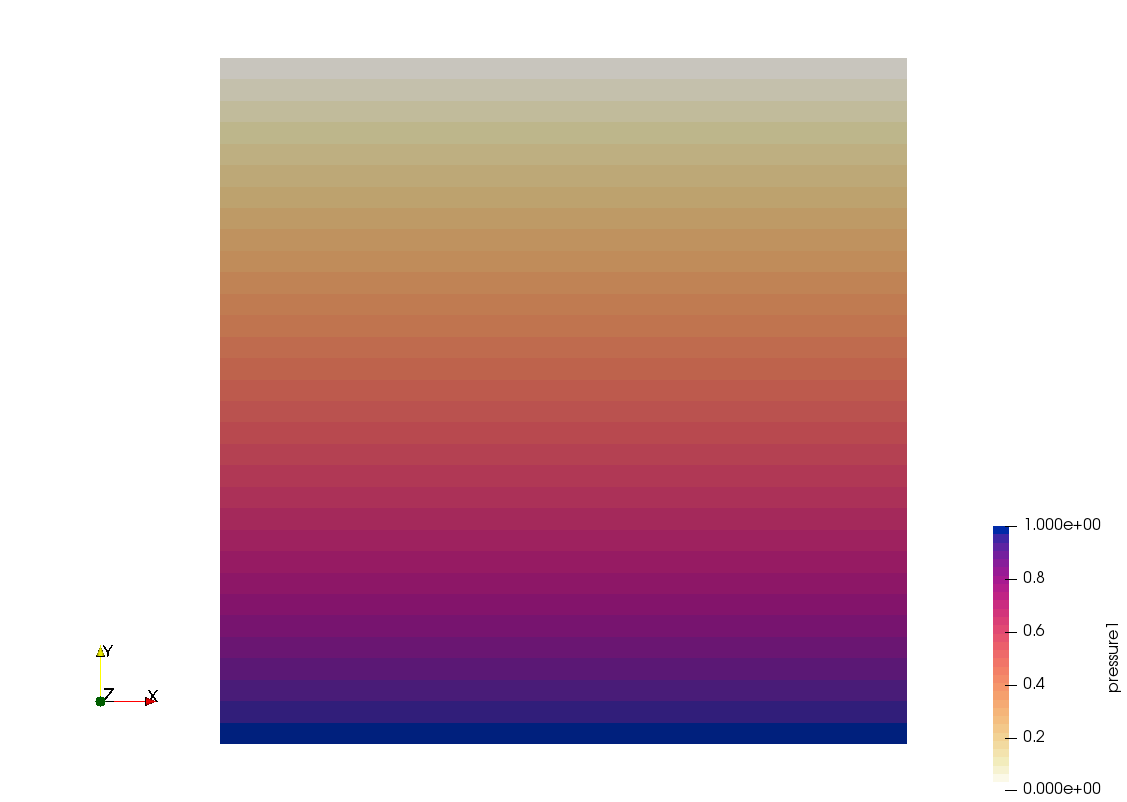
\includegraphics[width=5.7cm]{python_codes/fieldstone_119/results/exp1/p1}
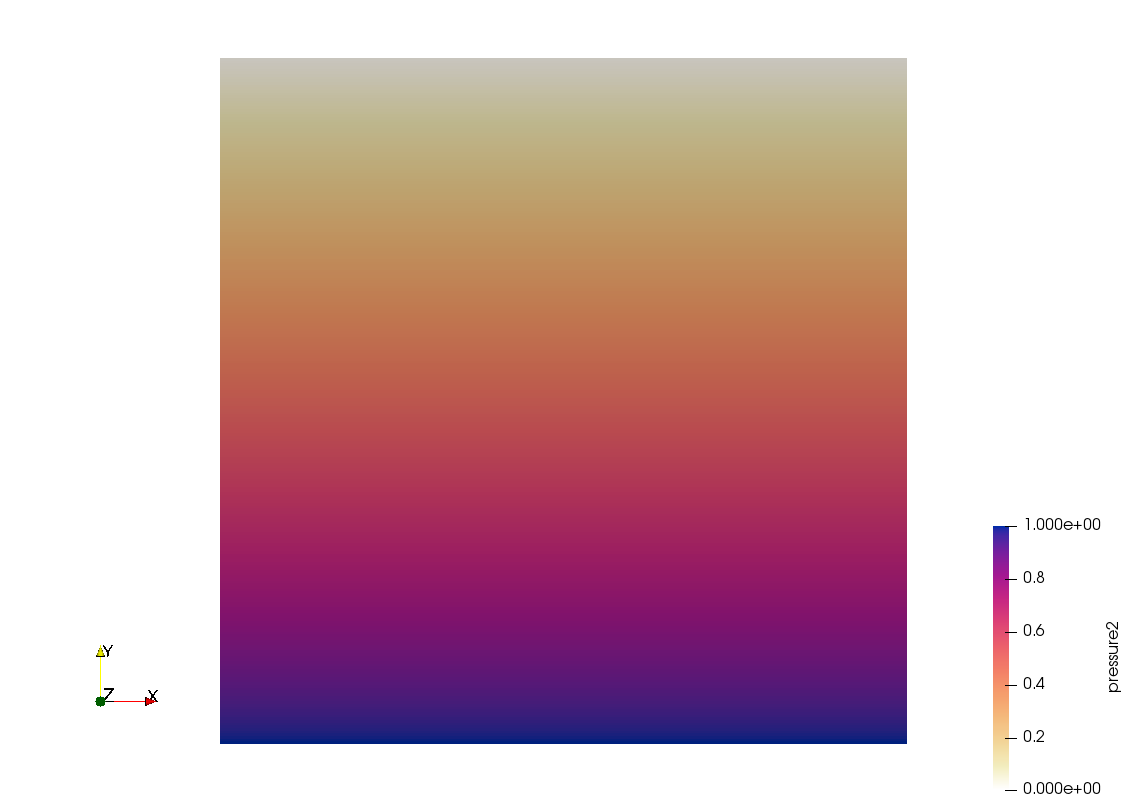
\includegraphics[width=5.7cm]{python_codes/fieldstone_119/results/exp1/p2}
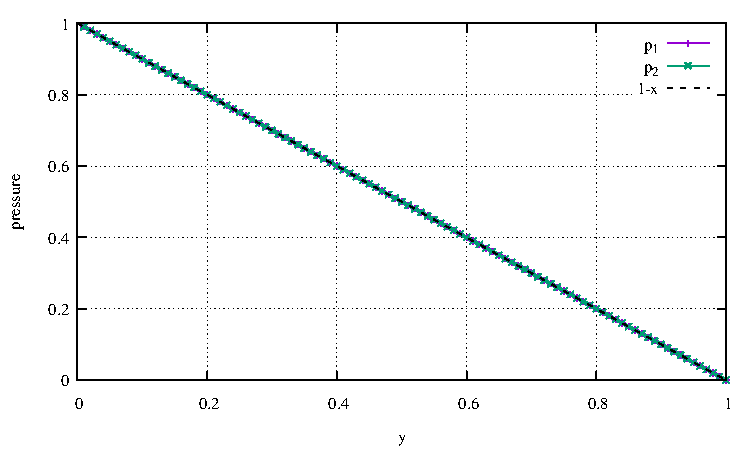
\includegraphics[width=5.7cm]{python_codes/fieldstone_119/results/exp1/profile.pdf}\\
{\captionfont Left: $p_1$; Right: $p_2$. Resolution 100$\times$100.}
\end{center}

We find that pressures $p_1$ and $p_2$ are identical.
\begin{center}
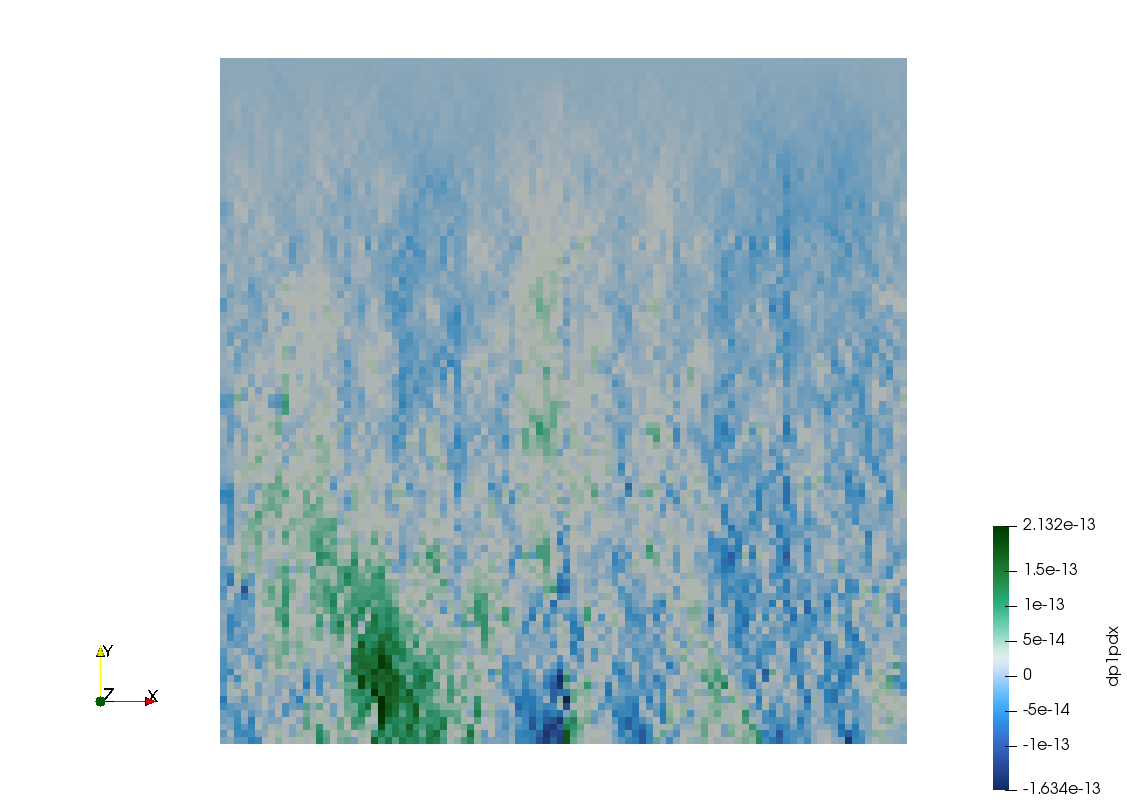
\includegraphics[width=4cm]{python_codes/fieldstone_119/results/exp1/dp1dx}
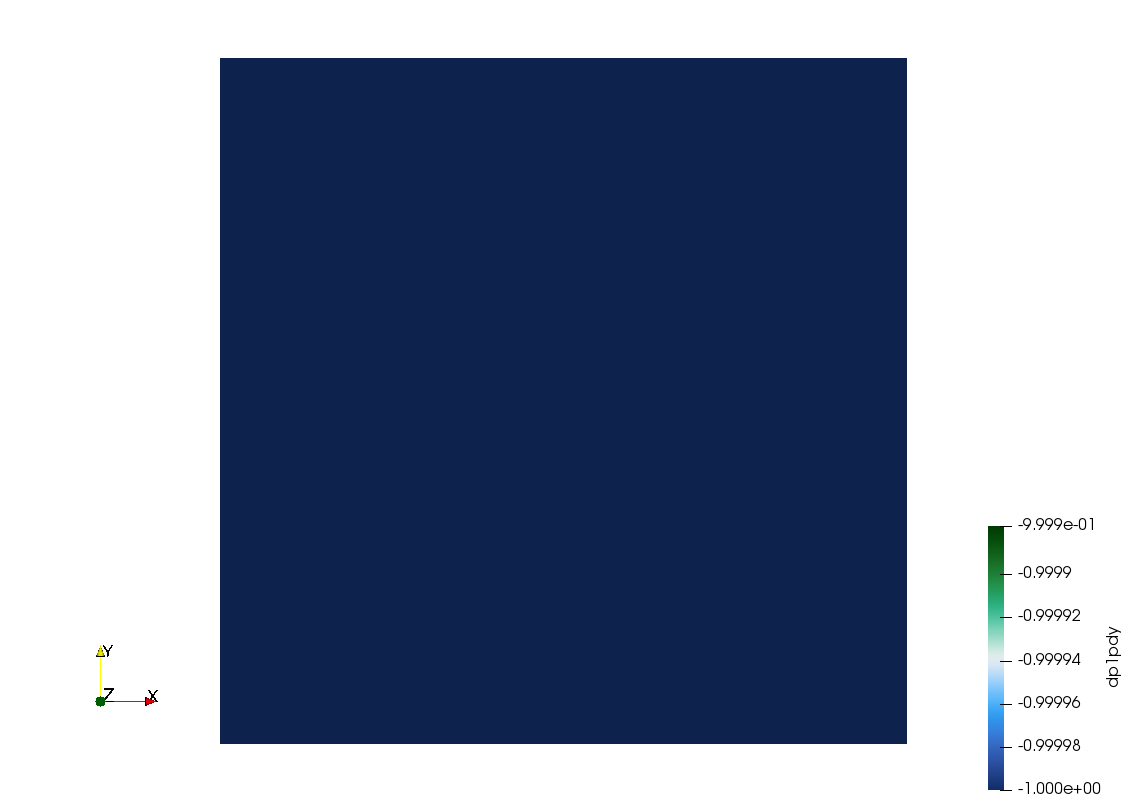
\includegraphics[width=4cm]{python_codes/fieldstone_119/results/exp1/dp1dy}
\includegraphics[width=4cm]{python_codes/fieldstone_119/results/exp1/dp2dx}
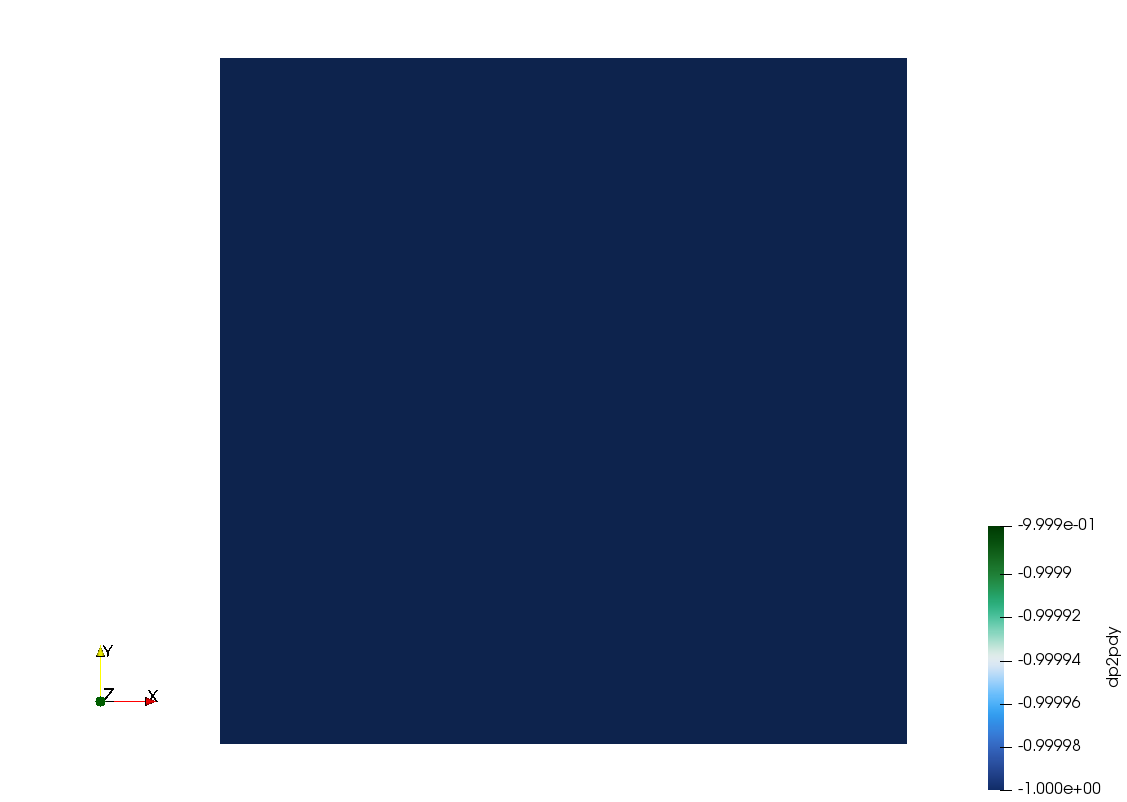
\includegraphics[width=4cm]{python_codes/fieldstone_119/results/exp1/dp2dy}\\
{\captionfont 
Pressure gradients from left to right: $\partial_xp_1$, $\partial_yp_1$, $\partial_xp_2$, $\partial_yp_2$. 
Resolution 100$\times$100.}
\end{center}

%------------------------------------------------------------------------------
\subsection*{Experiment \#2 - benchmark}

Same setup as Experiment \# 1, but now $\rho=1$ in the top half of the domain and $\rho=2$ in the bottom half.

\begin{center}
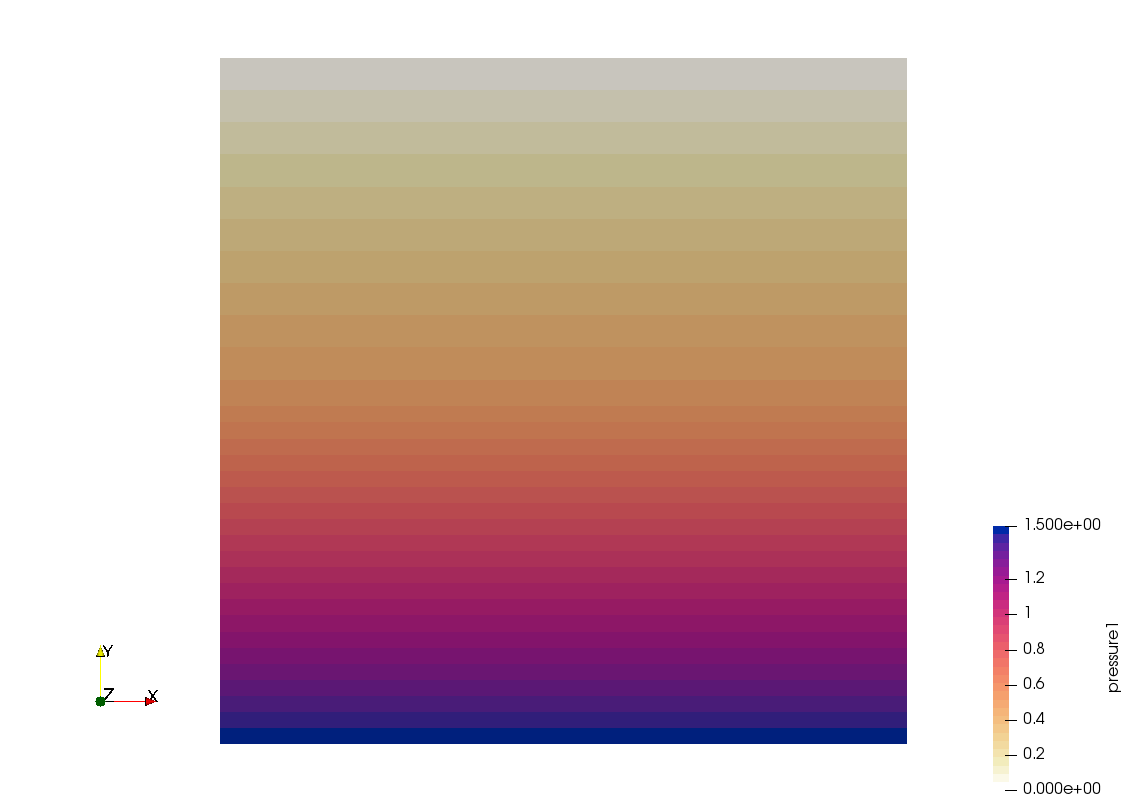
\includegraphics[width=5.7cm]{python_codes/fieldstone_119/results/exp2/p1}
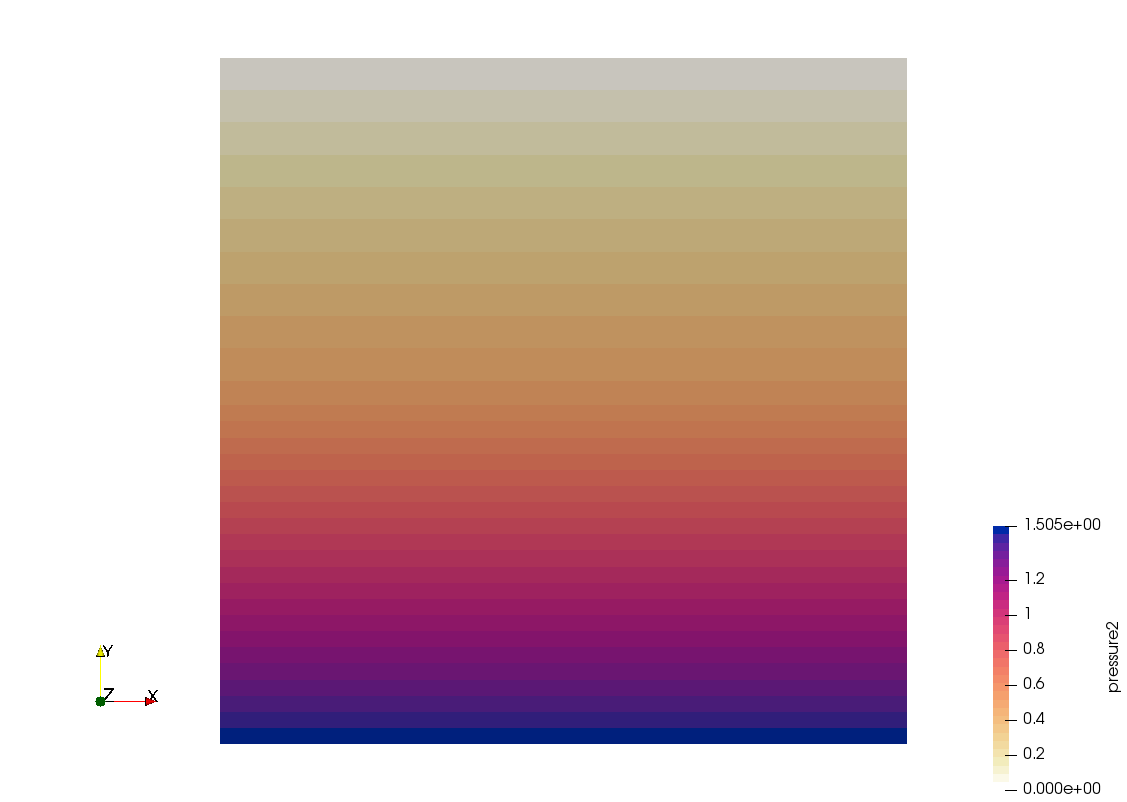
\includegraphics[width=5.7cm]{python_codes/fieldstone_119/results/exp2/p2}
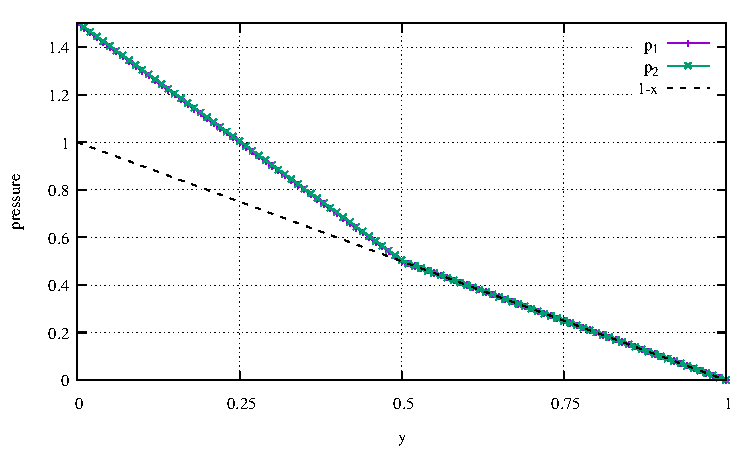
\includegraphics[width=5.7cm]{python_codes/fieldstone_119/results/exp2/profile.pdf}\\
{\captionfont Left: $p_1$; Right: $p_2$. Resolution 100$\times$100.}
\end{center}

We find that pressures $p_1$ and $p_2$ are identical.

\begin{center}
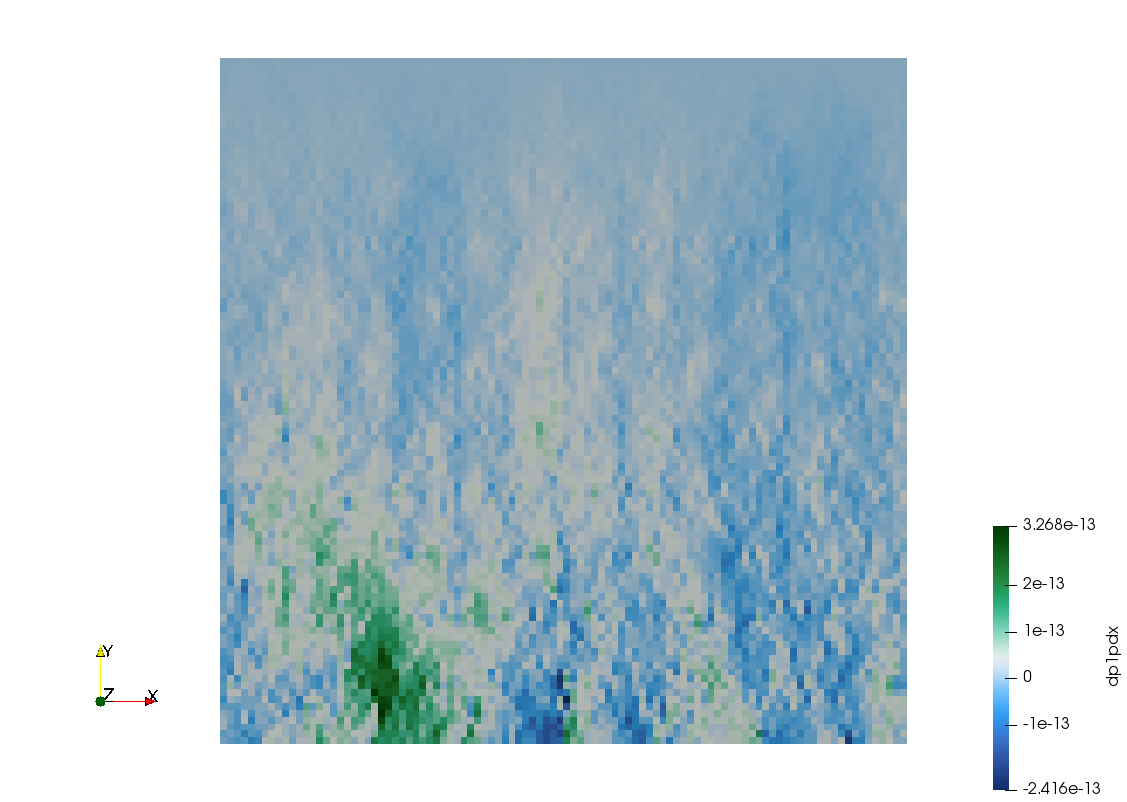
\includegraphics[width=4cm]{python_codes/fieldstone_119/results/exp2/dp1dx}
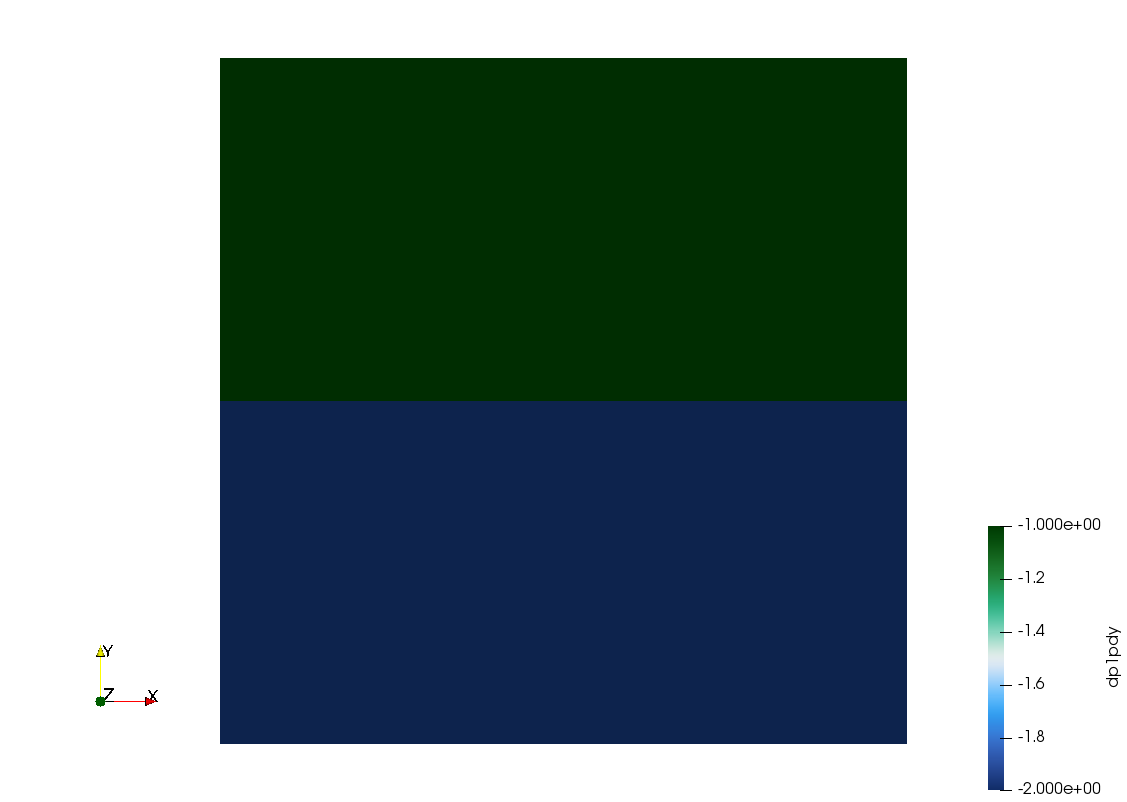
\includegraphics[width=4cm]{python_codes/fieldstone_119/results/exp2/dp1dy}
\includegraphics[width=4cm]{python_codes/fieldstone_119/results/exp2/dp2dx}
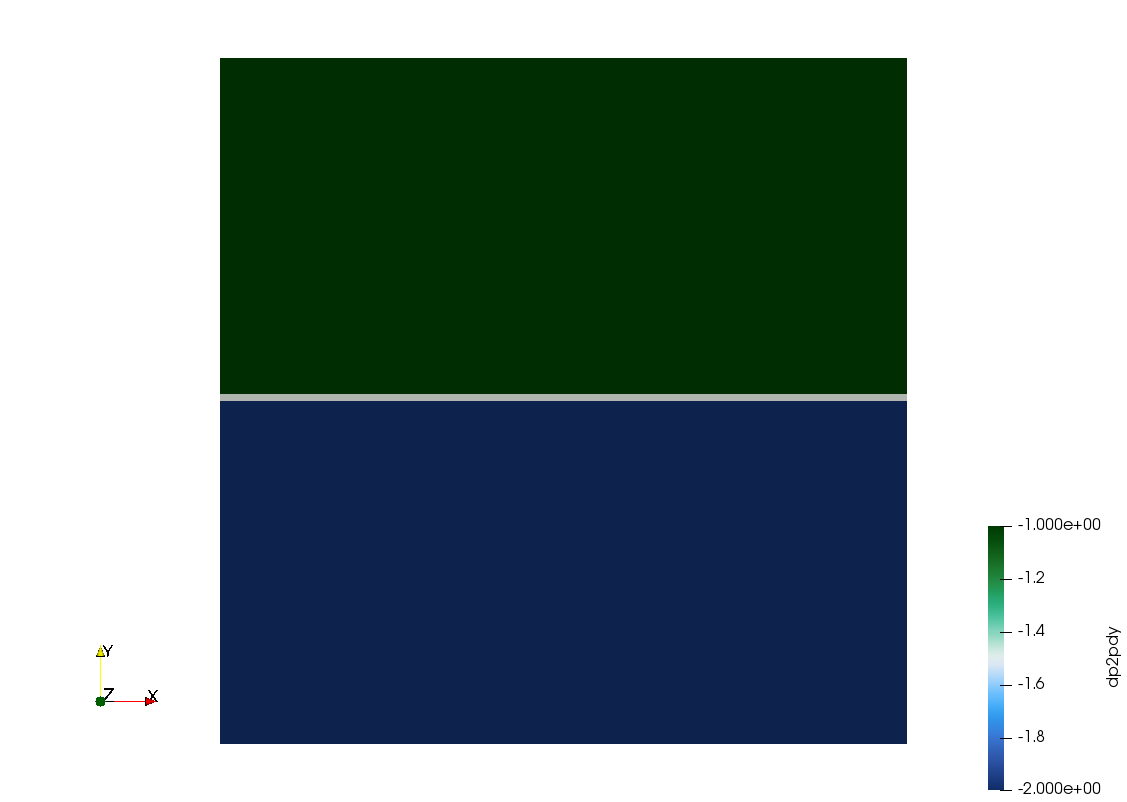
\includegraphics[width=4cm]{python_codes/fieldstone_119/results/exp2/dp2dy}\\
{\captionfont 
Pressure gradients from left to right: $\partial_xp_1$, $\partial_yp_1$, $\partial_xp_2$, $\partial_yp_2$. 
Resolution 100$\times$100.}
\end{center}

\newpage
%------------------------------------------------------------------------------
\subsection*{Experiment \#3}

Same setup as Experiment \# 1, but now $\rho=1$ in the left half of the domain and $\rho=2$ in the right half.

\begin{center}
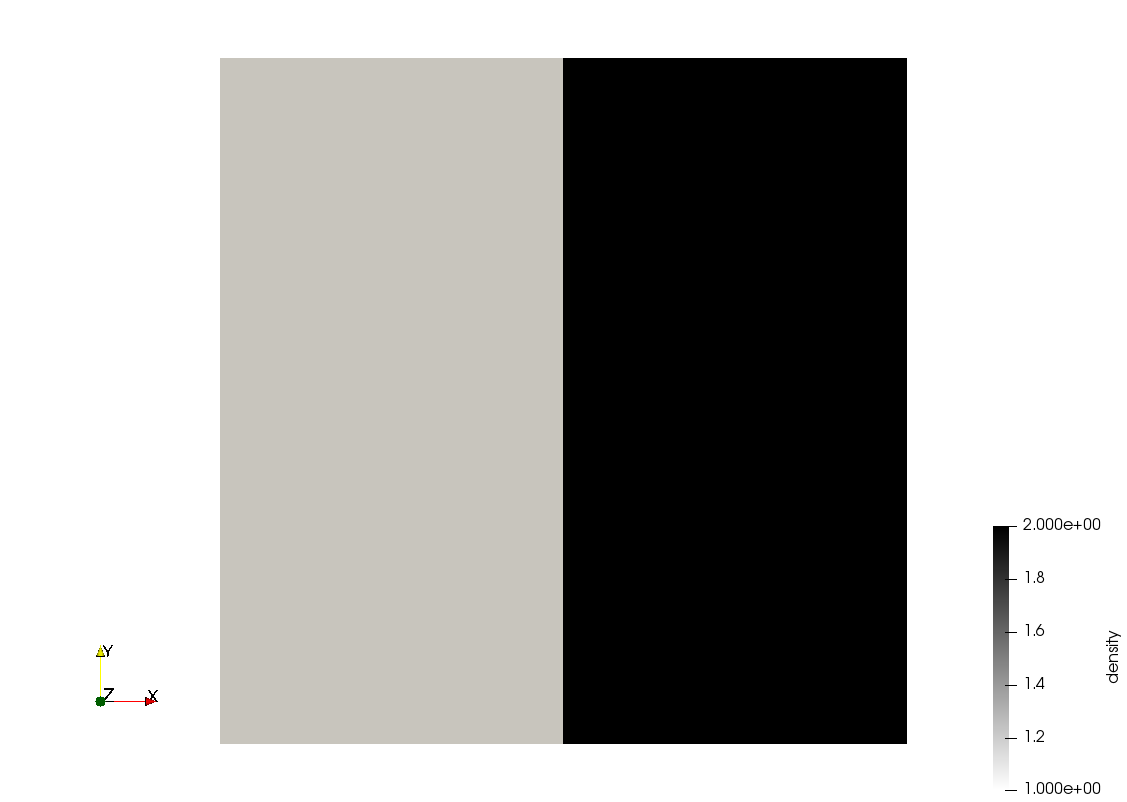
\includegraphics[width=5.6cm]{python_codes/fieldstone_119/results/exp3/rho}
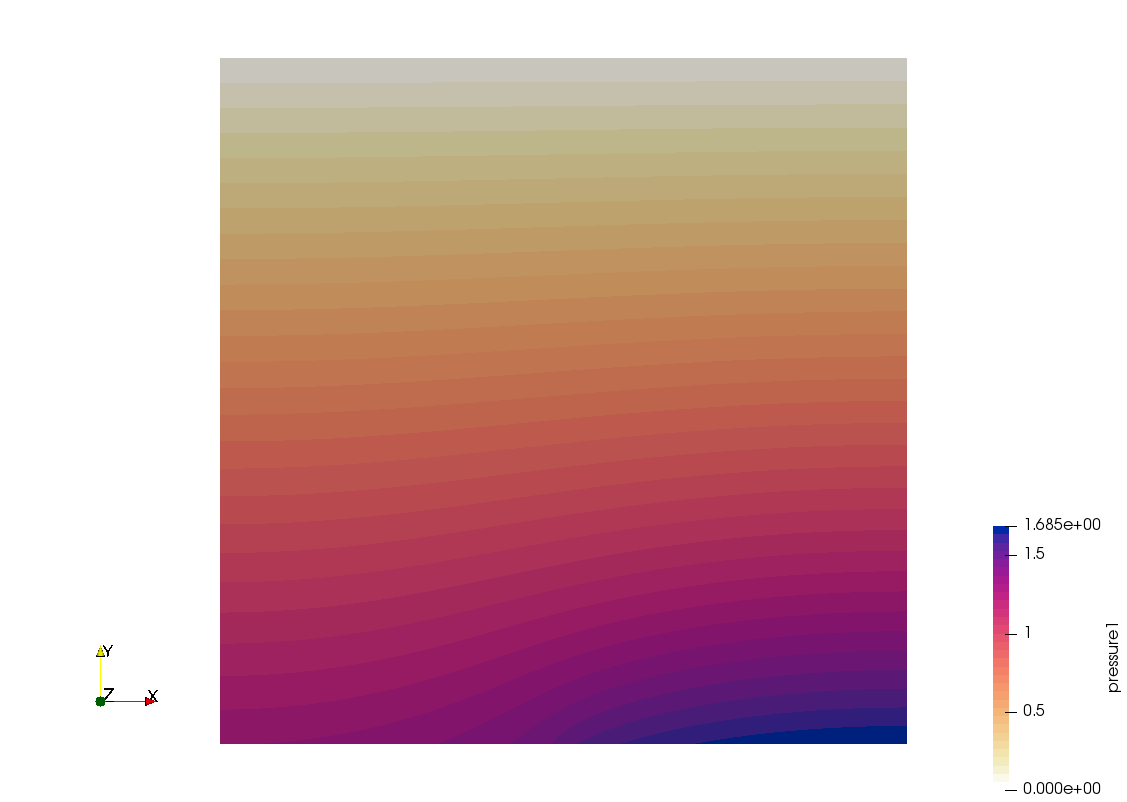
\includegraphics[width=5.6cm]{python_codes/fieldstone_119/results/exp3/p1}
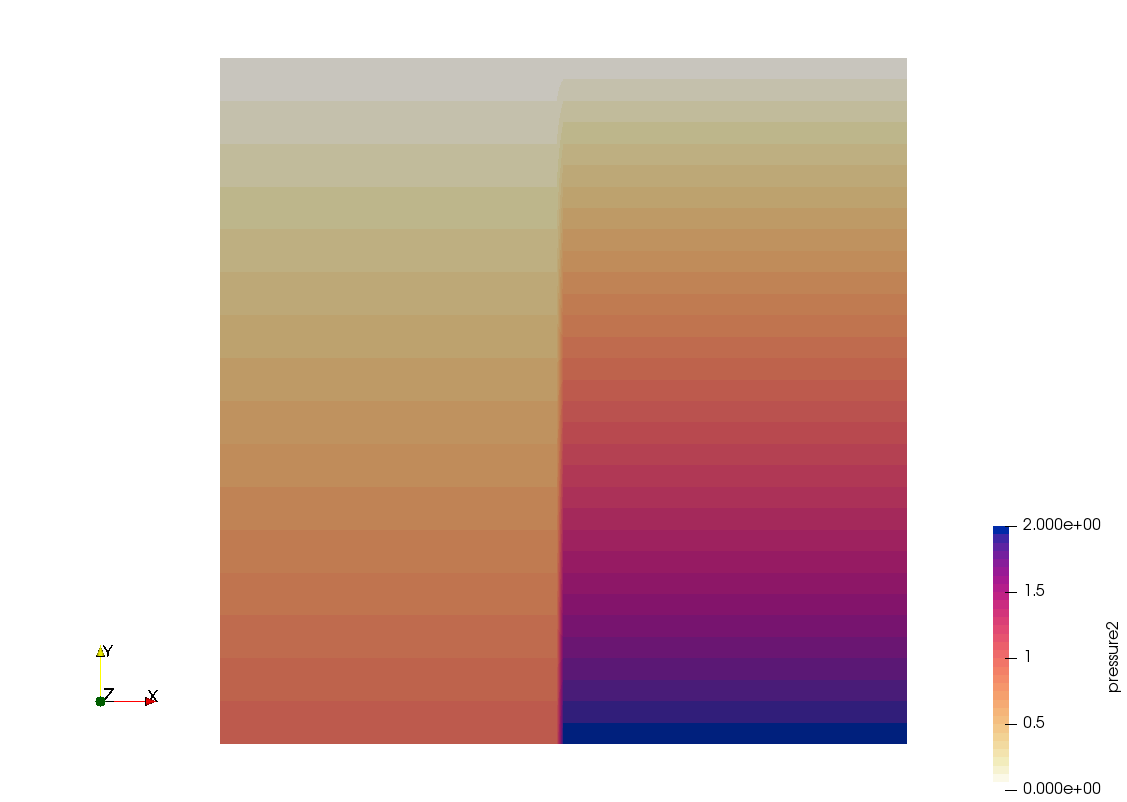
\includegraphics[width=5.6cm]{python_codes/fieldstone_119/results/exp3/p2}\\
{\captionfont Left: density; middle: $p_1$; Right: $p_2$. Resolution 100$\times$100.}
\end{center}

\begin{center}
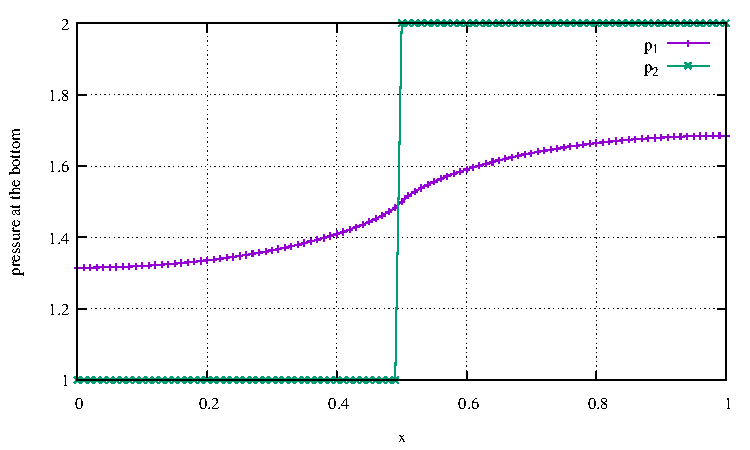
\includegraphics[width=5.7cm]{python_codes/fieldstone_119/results/exp3/bottom}
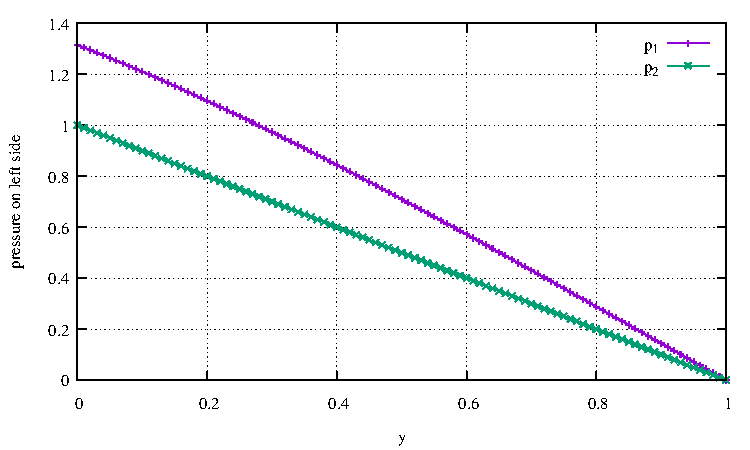
\includegraphics[width=5.7cm]{python_codes/fieldstone_119/results/exp3/left}
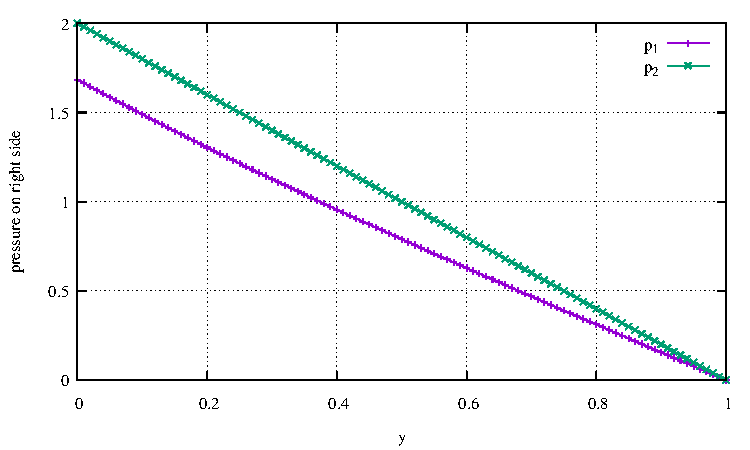
\includegraphics[width=5.7cm]{python_codes/fieldstone_119/results/exp3/right}\\
{\captionfont Pressure profiles at the bottom, left and right boundaries}
\end{center}

We find that pressures $p_1$ and $p_2$ are very different (pattern and amplitude). 

\begin{center}
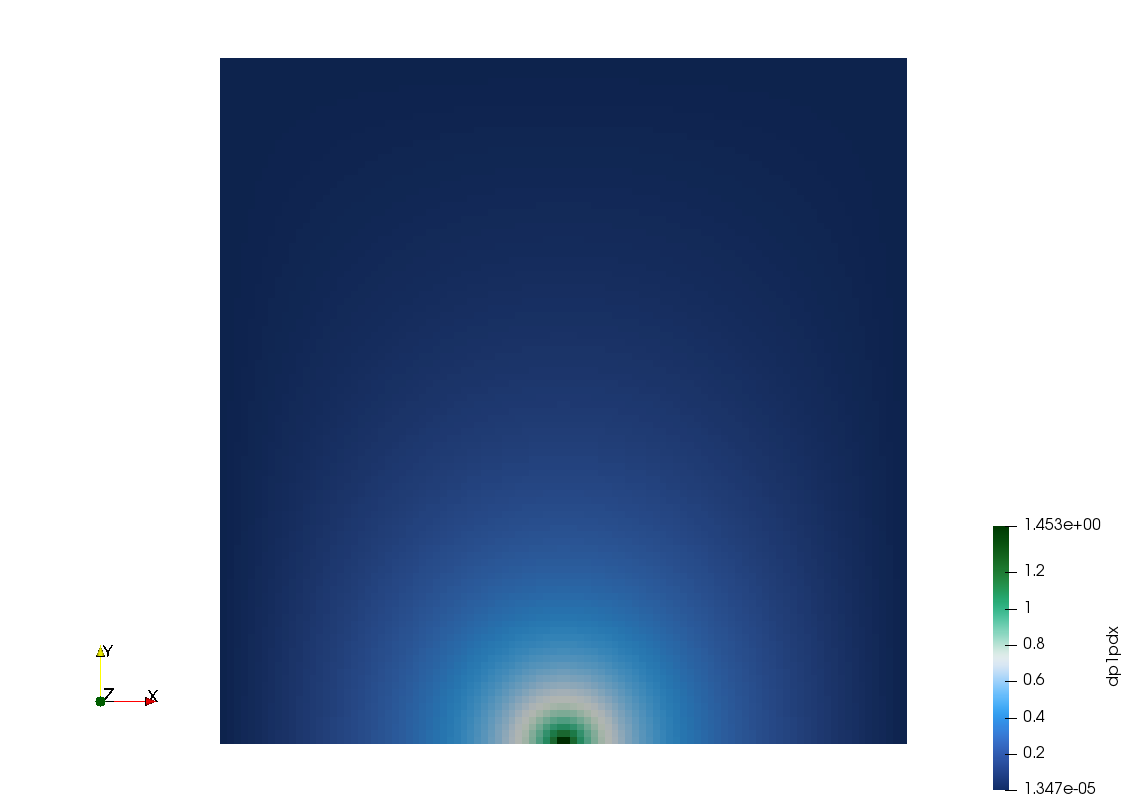
\includegraphics[width=4.2cm]{python_codes/fieldstone_119/results/exp3/dp1dx}
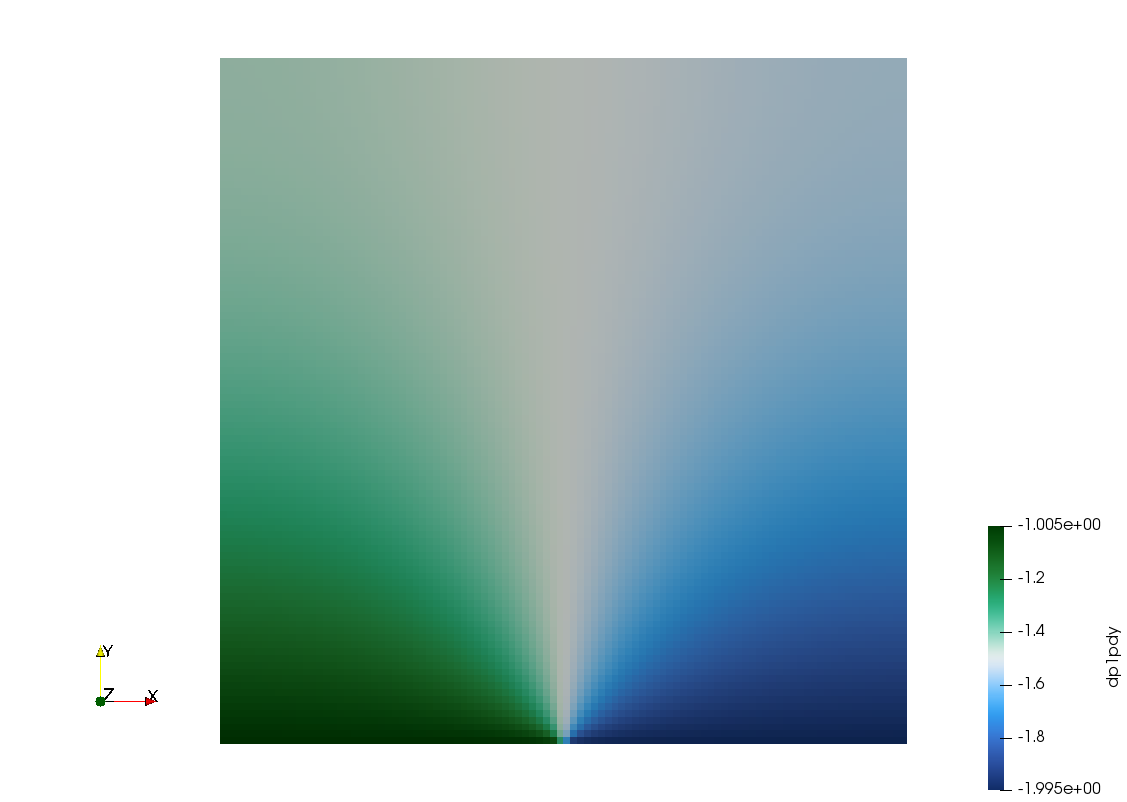
\includegraphics[width=4.2cm]{python_codes/fieldstone_119/results/exp3/dp1dy}
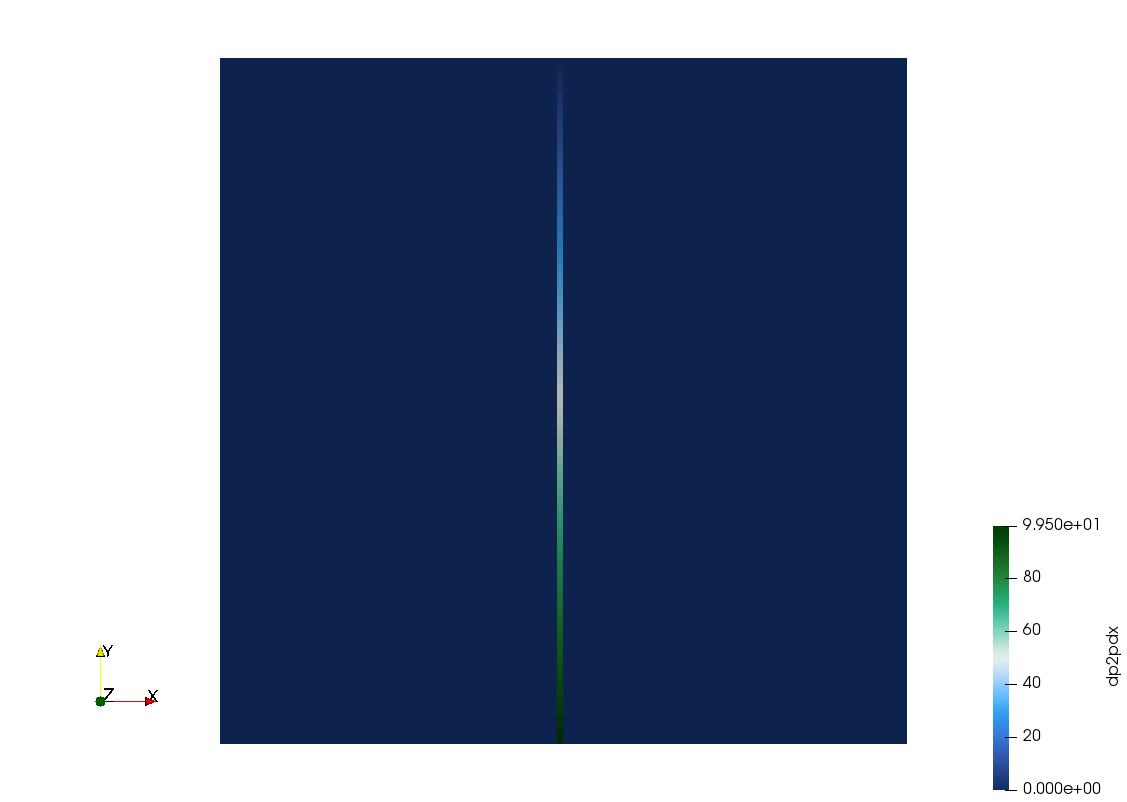
\includegraphics[width=4.2cm]{python_codes/fieldstone_119/results/exp3/dp2dx}
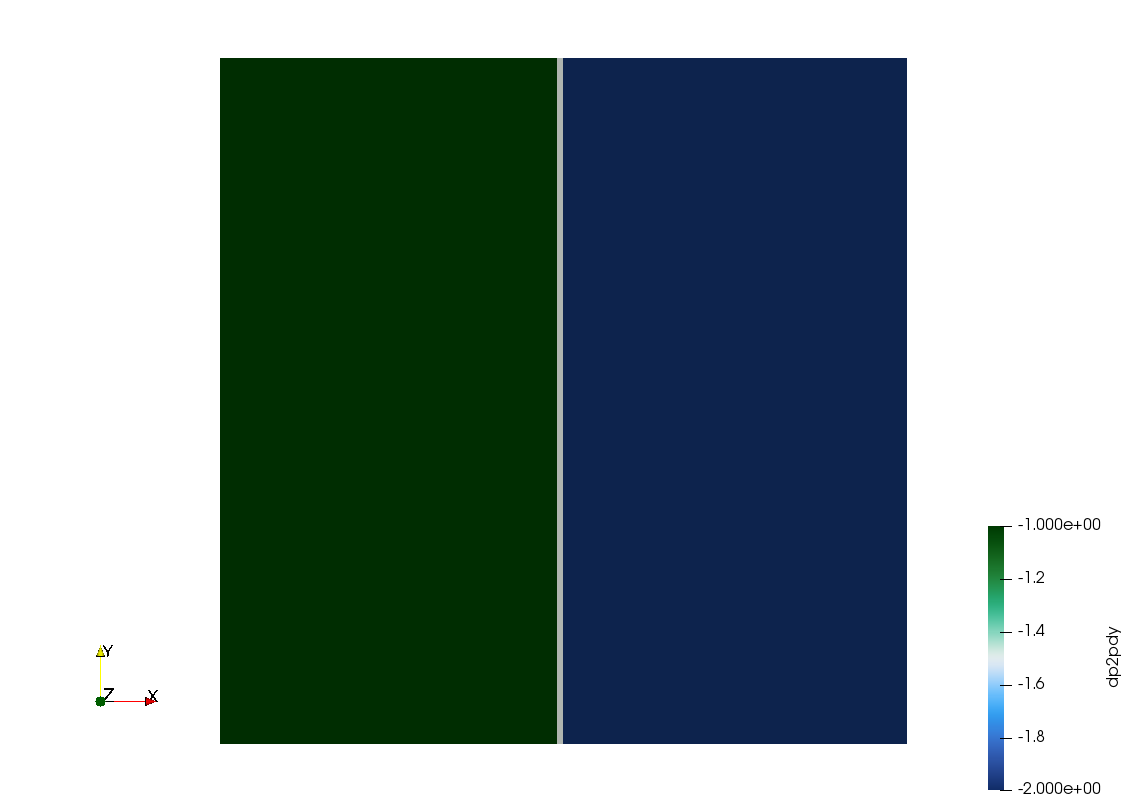
\includegraphics[width=4.2cm]{python_codes/fieldstone_119/results/exp3/dp2dy}\\
{\captionfont Pressure gradients from left to right: $\partial_xp_1$, $\partial_yp_1$, $\partial_xp_2$, $\partial_yp_2$. 
Resolution 100$\times$100.}
\end{center}

Obviously we do not have $\vec{\nabla}p=-\rho\vec{g}$ for the pressure obtained with 
the Poisson equation!

\newpage
%------------------------------------------------------------------------------
\subsection*{Experiment \#4}

In this experiment the density is 1 except in a centered disc of radius 0.25 in which it is 2, 
and $g=10$. I have approached A. Jourdon and asked him to carry out this experiment 
with the code used in his paper. 

\begin{center}
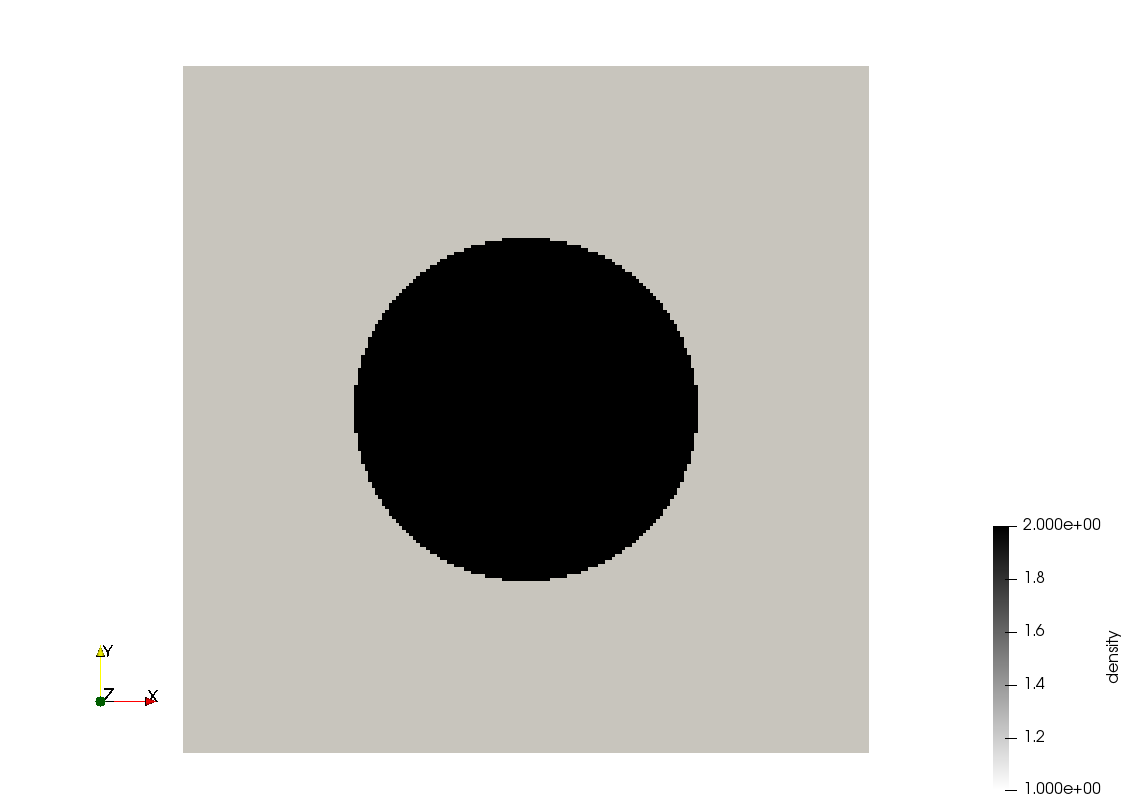
\includegraphics[width=7cm]{python_codes/fieldstone_119/results/exp4/rho}
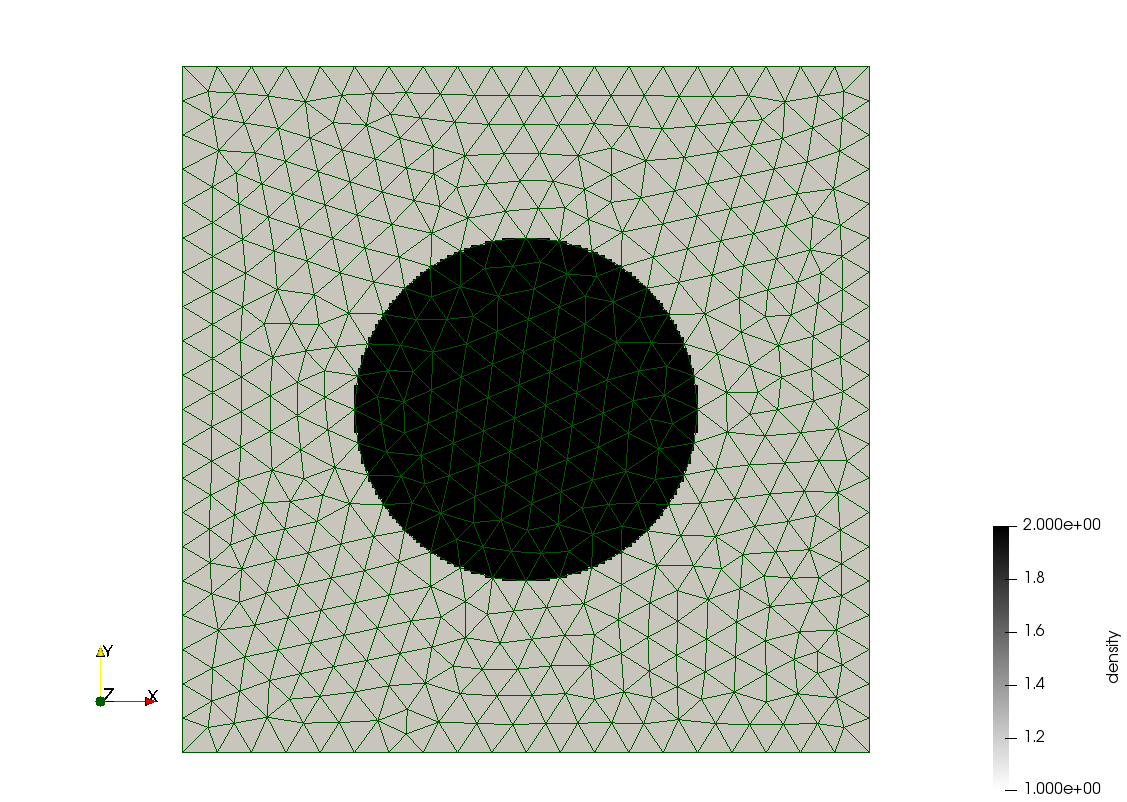
\includegraphics[width=7cm]{python_codes/fieldstone_119/results/exp4/rho_joma22_mesh}\\
{\captionfont Left: density field on 200x200 mesh. right: mesh used by Jourdon with 
my density field superimposed.}
\end{center}

\begin{center}
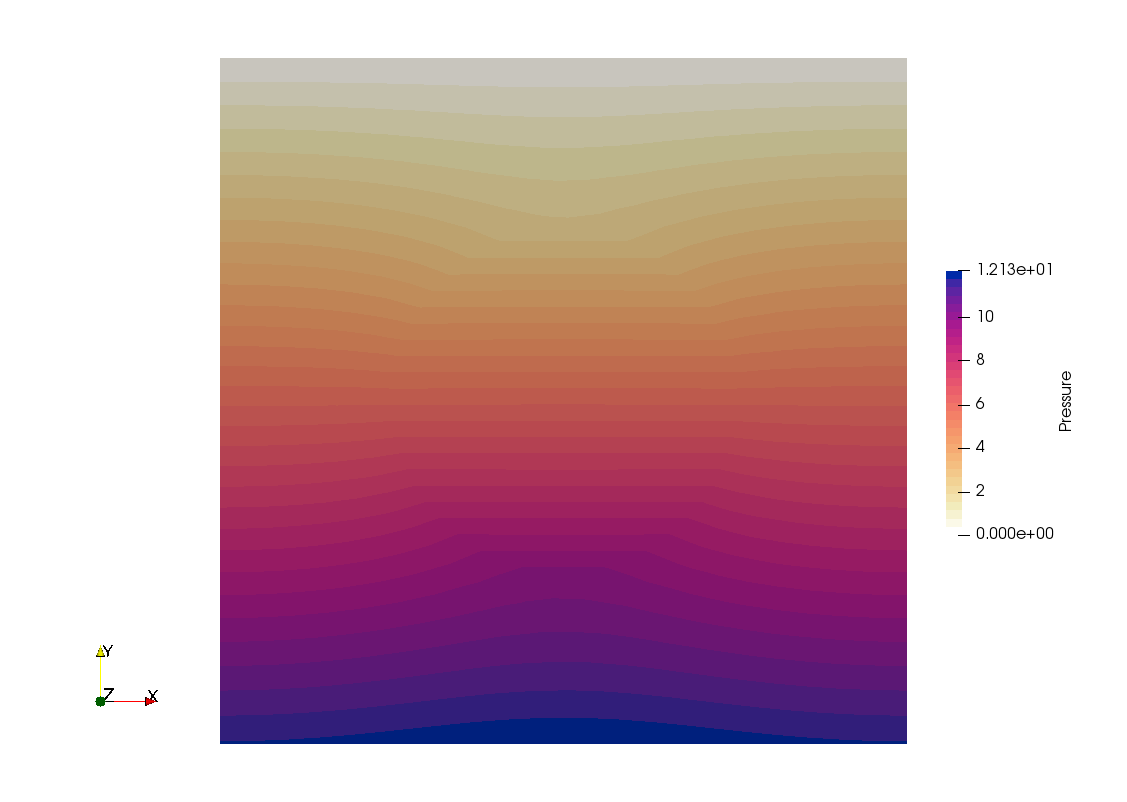
\includegraphics[width=5.7cm]{python_codes/fieldstone_119/results/exp4/p_joma22}
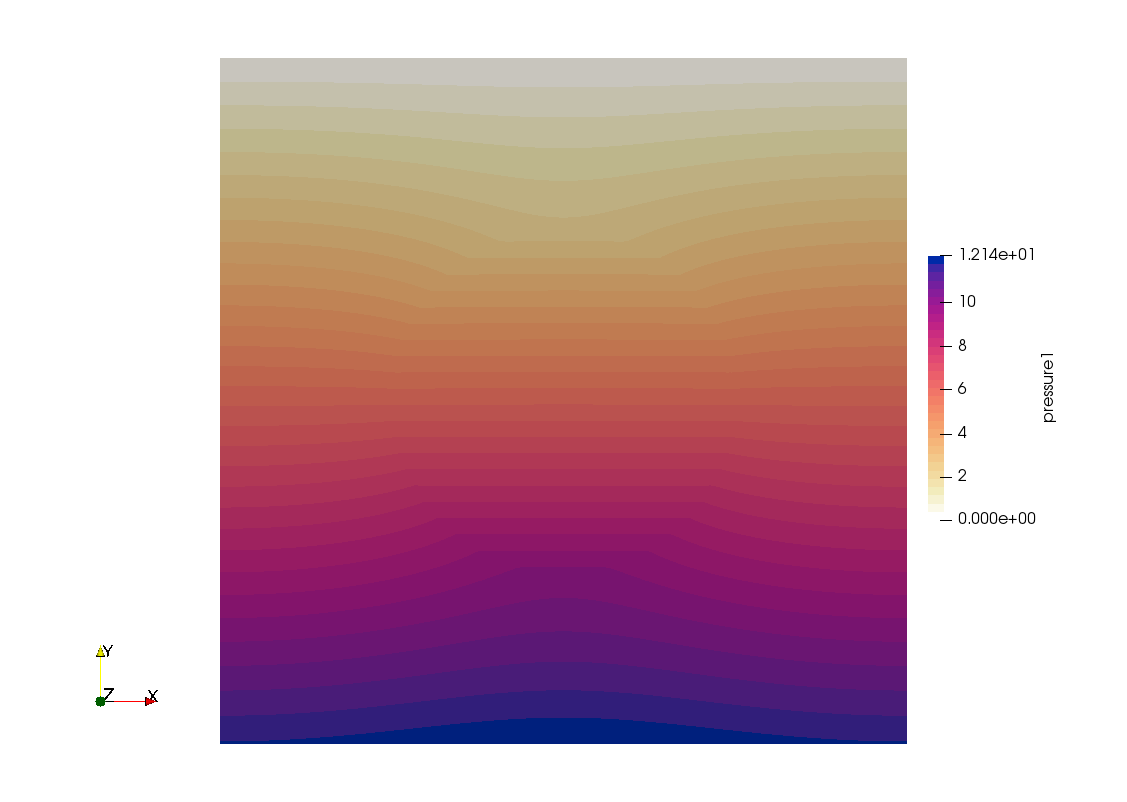
\includegraphics[width=5.7cm]{python_codes/fieldstone_119/results/exp4/p1}
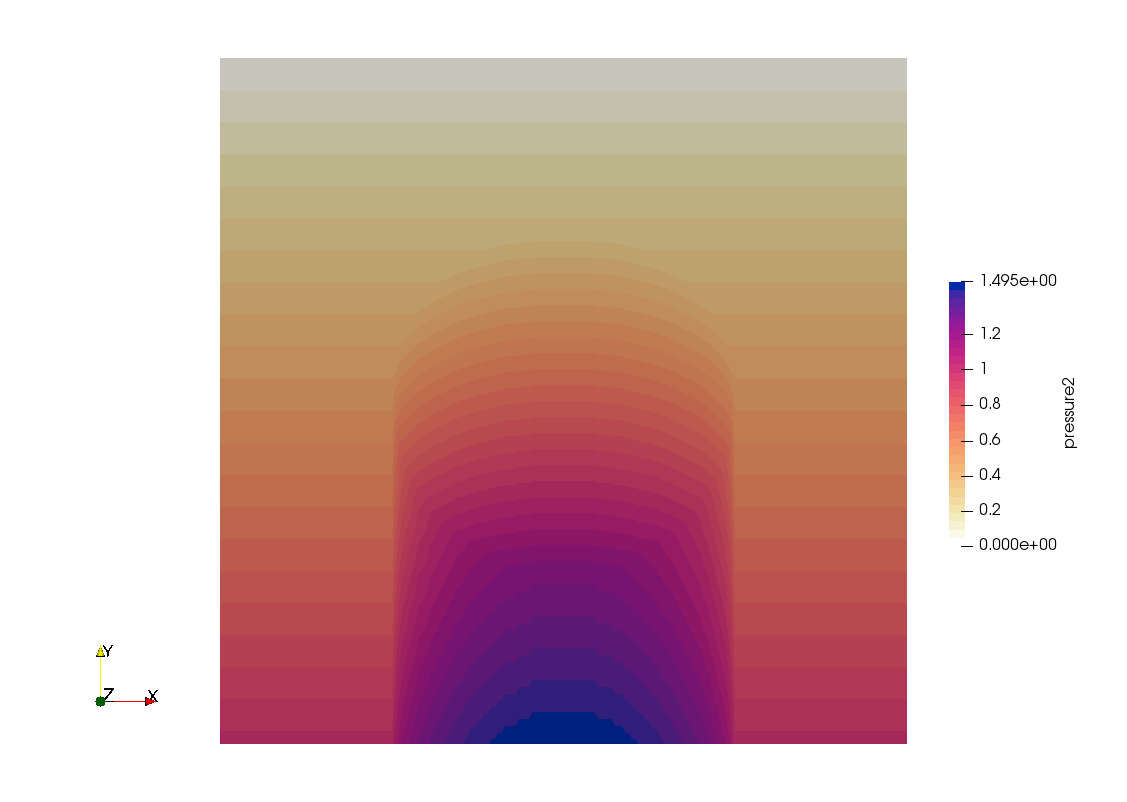
\includegraphics[width=5.7cm]{python_codes/fieldstone_119/results/exp4/p2}\\
{\captionfont Left: pressure from Jourdon; Middle: $p_1$; Right: $p_2$. Resolution 200$\times$200.}
\end{center}

\begin{center}
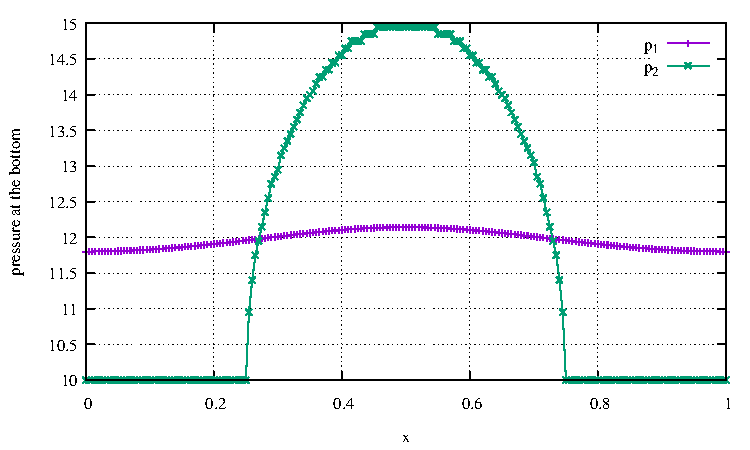
\includegraphics[width=7.5cm]{python_codes/fieldstone_119/results/exp4/bottom}
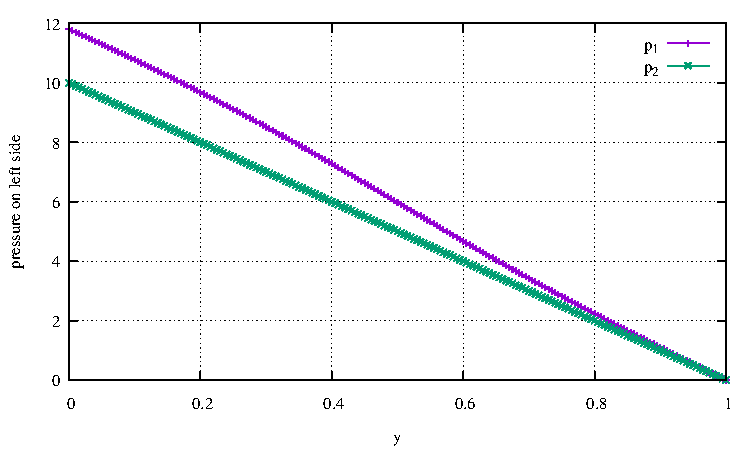
\includegraphics[width=7.5cm]{python_codes/fieldstone_119/results/exp4/left}\\
{\captionfont Pressures $p_1$ and $p_2$ at the bottom and left boundary.}
\end{center}

We find that pressures $p_1$ and $p_2$ are again very different (pattern and amplitude), but 
we find that $p_1$ and the results sent by Jourdon are identical (which validates my implementation):

\begin{center}
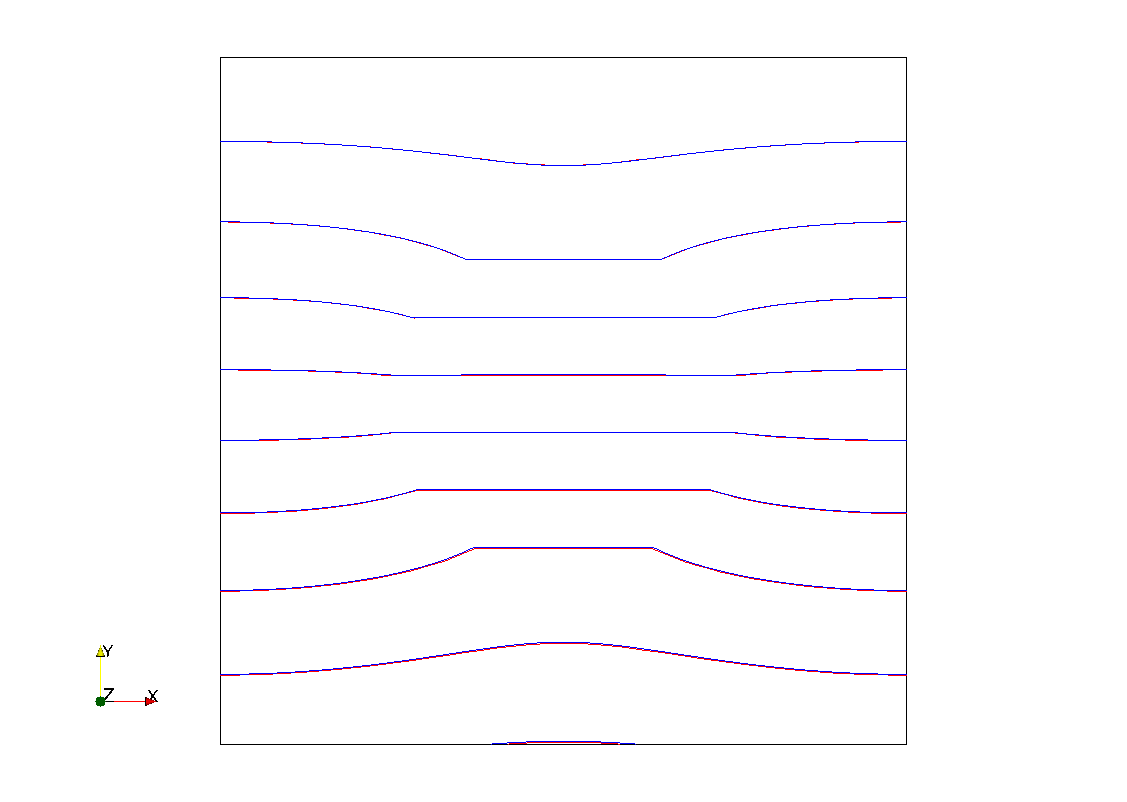
\includegraphics[width=7cm]{python_codes/fieldstone_119/results/exp4/p1_both}\\
{\captionfont Pressure isocontours for both pressures obtained with this \stone and Jourdon's code.}
\end{center}
 
\begin{center}
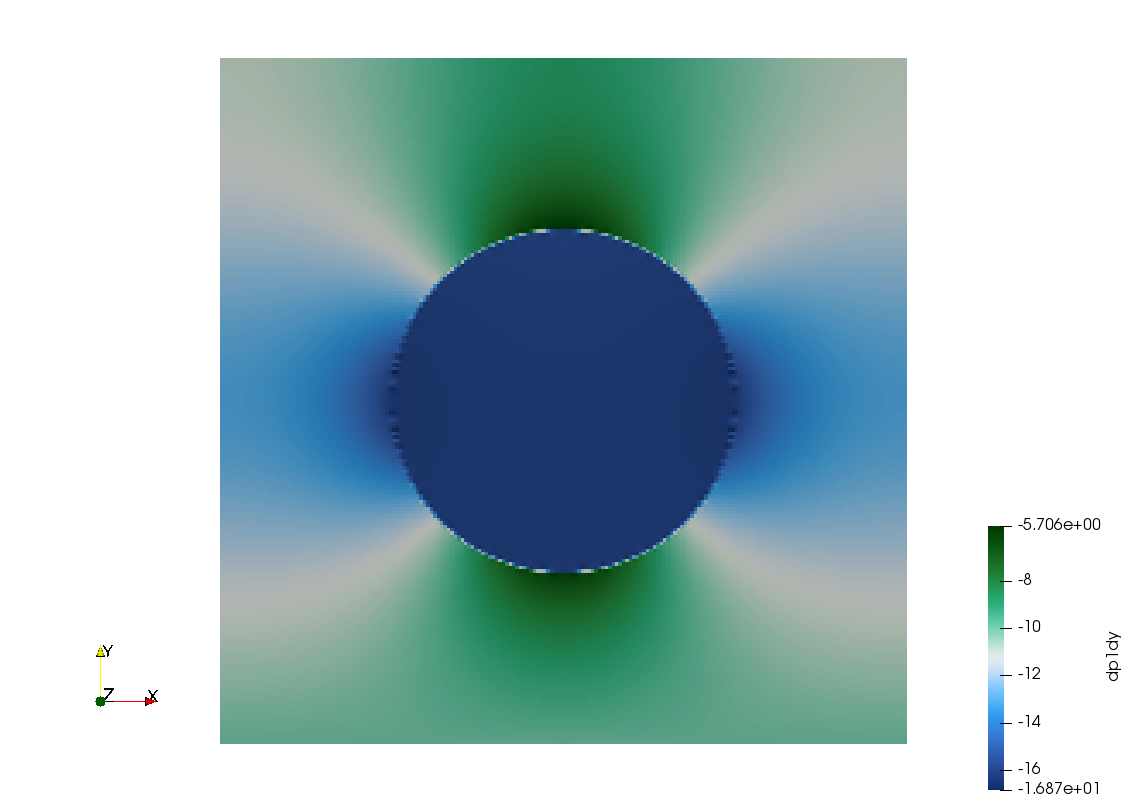
\includegraphics[width=7cm]{python_codes/fieldstone_119/results/exp4/dp1dy}
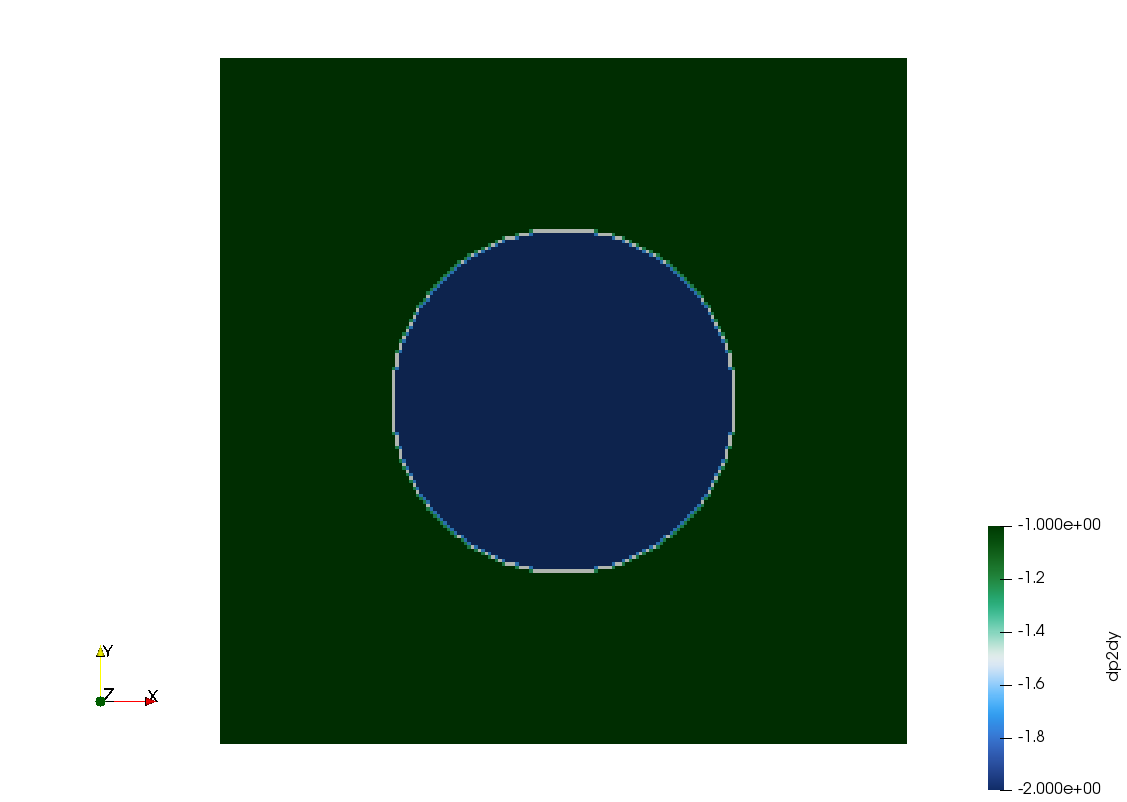
\includegraphics[width=7cm]{python_codes/fieldstone_119/results/exp4/dp2dy}\\
{\captionfont Pressure gradients. Left: $\partial_yp_1$; Right: $\partial_yp_2$. Resolution 200$\times$200.}
\end{center}

Obviously we here again do not have $\vec{\nabla}p=-\rho\vec{g}$ for the pressure obtained with 
the Poisson equation!
%The pressure at the bottom for $x<0.25$ should be constant and equal to 10, but this is not 
%the case for the Poisson pressure, so it is not a lithostatic pressure. Only $p_2$ is. 

\newpage
%------------------------------------------------------------------------------
\subsection*{Experiment \#5}

In this experiment the density is 1 except in a centered disc of radius 0.1 in which it is 10, 
and $g=10$. 
I have also written a $Q_2\times Q_1$ FE Stokes solver so as to look at the computed 
full pressure. Viscosity of the ball is 100 while viscosity of the fluid is 1. 
Free slip boundary conditions are prescribed on the sides and on the bottom. 
Either the top surface is free, either free slip is also imposed in 
conjunction with a zero average surface pressure normalisation.

\begin{center}
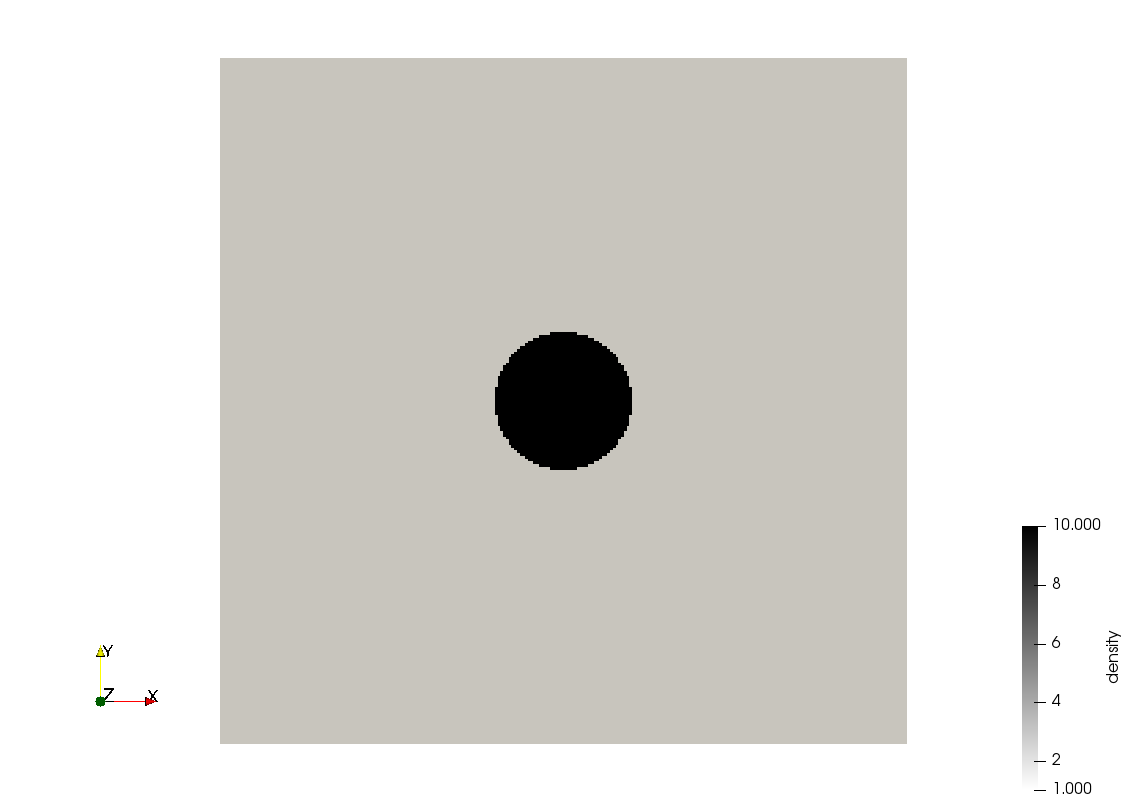
\includegraphics[width=5.7cm]{python_codes/fieldstone_119/results/exp5/rho}
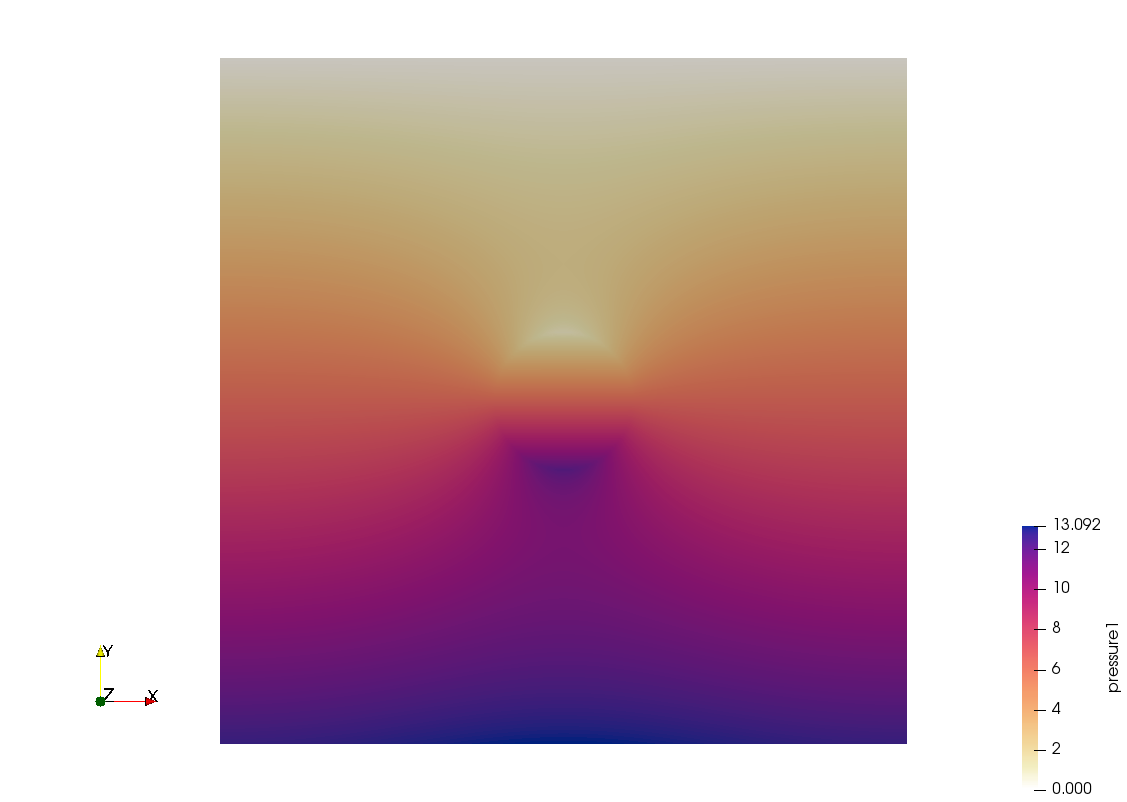
\includegraphics[width=5.7cm]{python_codes/fieldstone_119/results/exp5/p1}
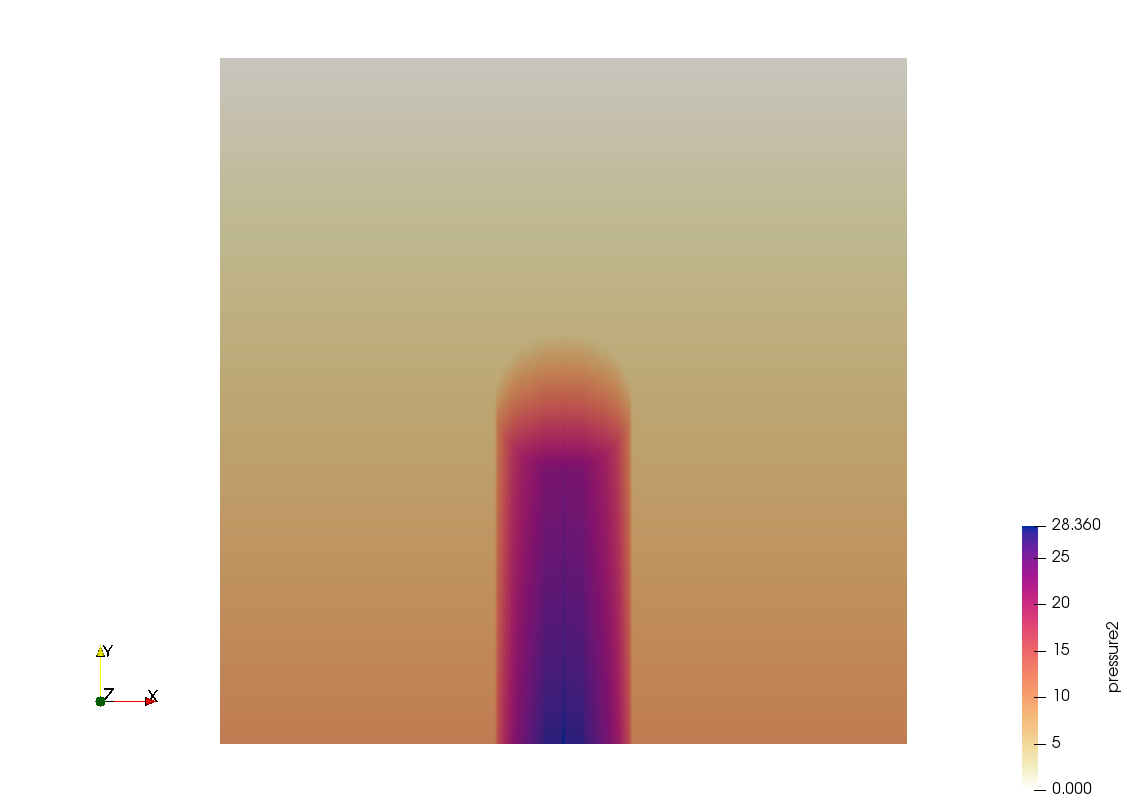
\includegraphics[width=5.7cm]{python_codes/fieldstone_119/results/exp5/p2}\\
{\captionfont Left: density field on 100x100 mesh. Middle: $p_1$ pressure; Right: $p_2$ pressure.} 
\end{center}

We find that for this example the pressure $p_1$ is closer to the full pressure than $p_2$:
\begin{center}
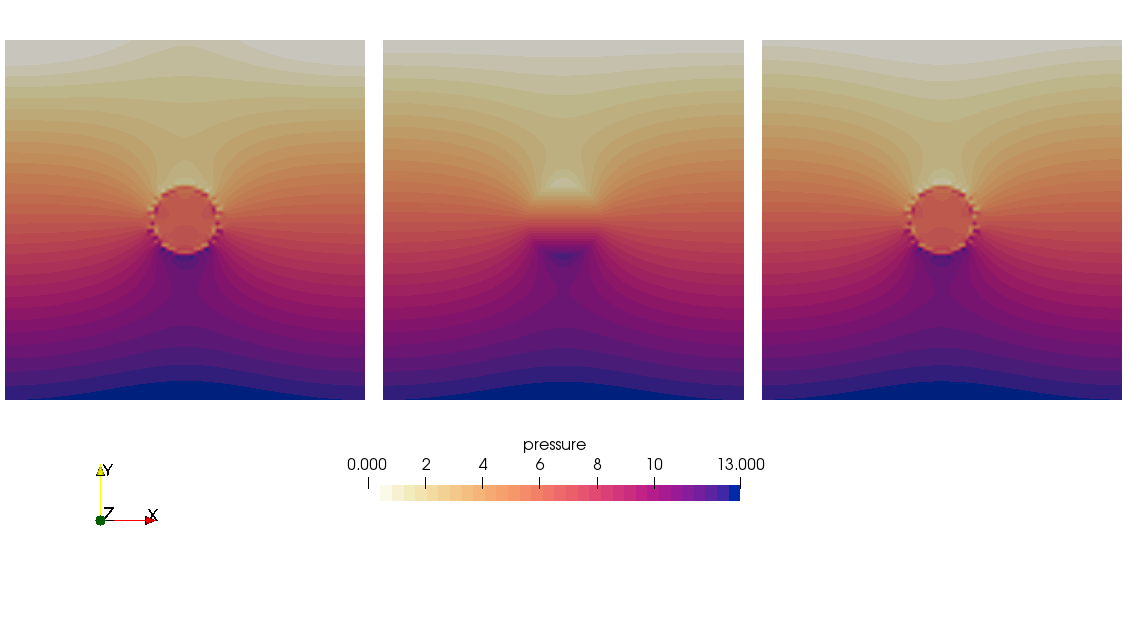
\includegraphics[width=7cm]{python_codes/fieldstone_119/results/exp5/comp1}
\hspace{0.5cm}
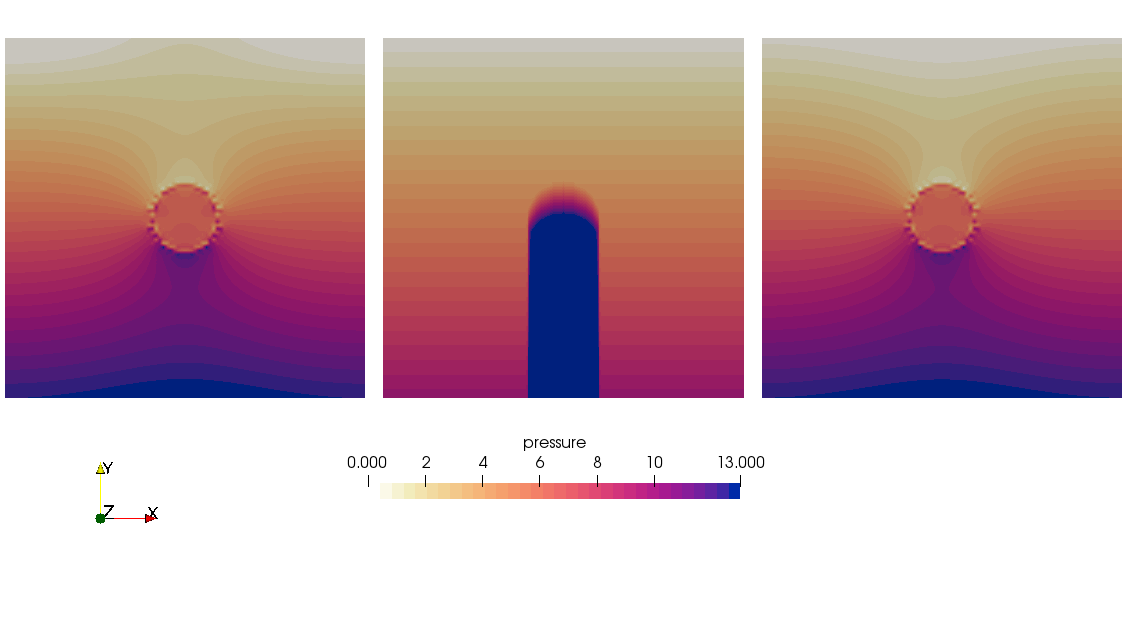
\includegraphics[width=7cm]{python_codes/fieldstone_119/results/exp5/comp2}\\
{\captionfont Left panel: pressure $p_1$ surrounded by full pressure fields (free surface
on the left, free slip on the right). Right panel: same with $p_2$ instead.}
\end{center}

Finally one can explore the effect of the aspect ratio:
\begin{center}
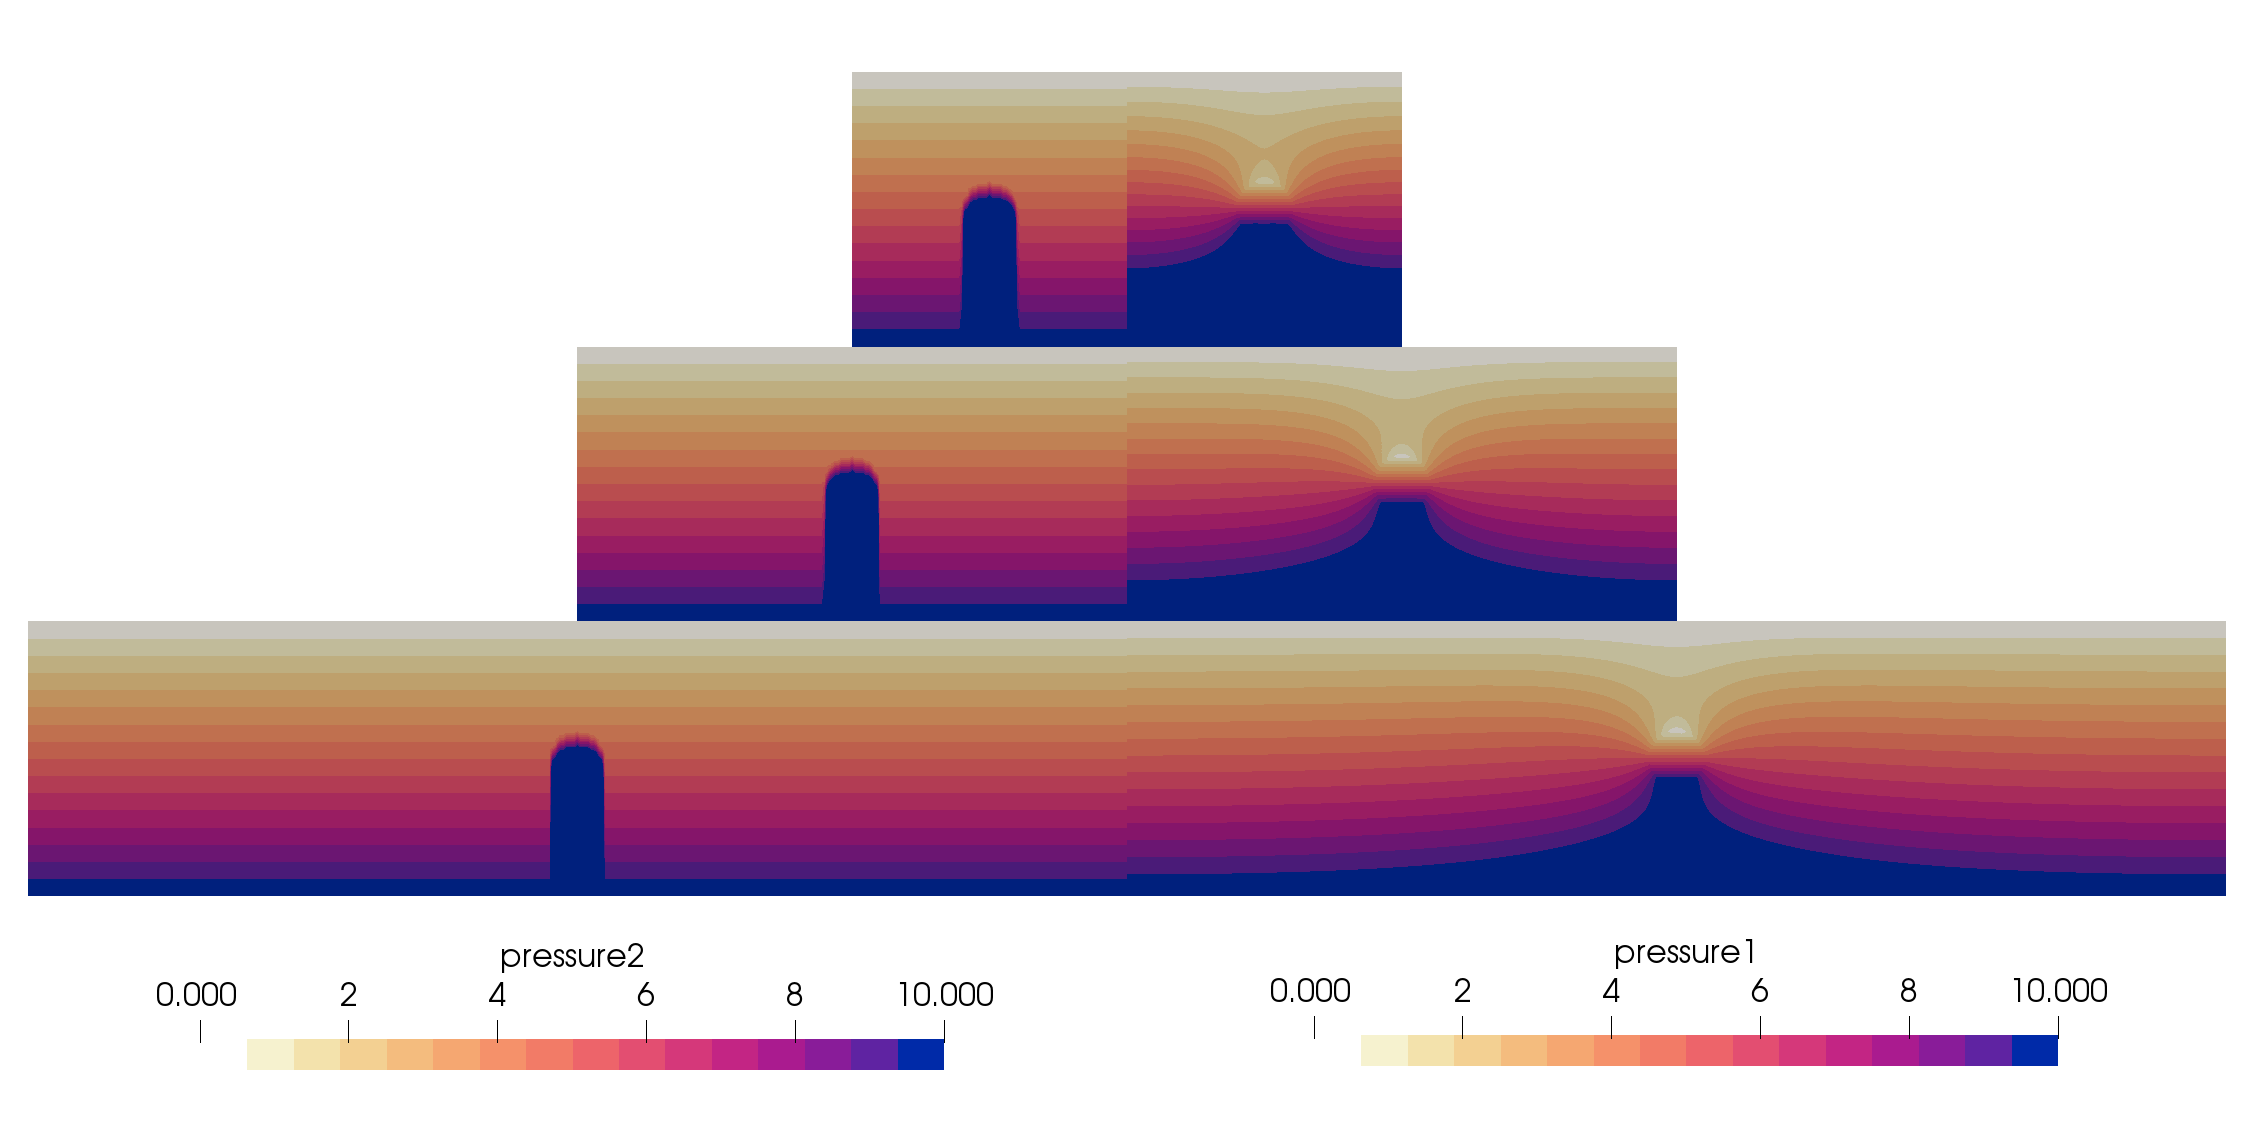
\includegraphics[width=14cm]{python_codes/fieldstone_119/results/exp5/all}\\
{\captionfont Left column: $p_1$ pressure; Right column: $p_2$ pressure. From 
top to bottom: aspect ratio 1:1, 2:1 and 4:1.}
\end{center}
We not-so-surprisingly find that 'far away from the source of buoyancy' 
pressure $p_1$ slowly becomes close to $p_2$. On the one hand, this means that 
if a long enough domain is used then prescribing $p_1$ or $p_2$ on the sides should not 
have much consequences. On the other hand, the conclusion of \textcite{chgv12} (2012) 
(the 'first' paper documenting the use of open boundary conditions in subduction modelling)
pertaining to the advantage of using such boundary conditions is then problematic: 
``Other advantages are the independence of the aspect ratio of the model domain, 
which allows for smaller models with increased resolution for modelling detail.''
Note that in this paper the authors do not specify how they compute the lithostatic pressure that 
they use for boundary conditions...

W.B.: ``This is again a case where $\rho g$ is not the gradient of a potential, 
and as a consequence there is no function $p(x,y)$ that would satisfy $\nabla p = \rho g$.
It {\it is} worth pointing out, I believe, that you don't actually solve
$\vec\nabla p = \rho \vec{g}$ in your experiments. You are solving $dp/dz = \rho g_z$
but these are not the same. If you have a vertical gravity vector, then the first equation 
implies $dp/dx=0$ (i.e., $p$ has no horizontal variation) but that is clearly not the case in your experiments.''
 








